\chapter{Evaluation and validation}
\label{ch:Evalutation-Validation}
This chapter presents the results and experiments conducted in this thesis. Section \ref{sec:Results-DCASE} describes the results of the experiments done on the \gls{DCASE} dataset (\ref{sub:DCASE-Task-Dataset}). In section \ref{sec:Results-Music}, the results of the experiments done on the music dataset (\ref{sub:Music-Dataset}) are described. Further, this chapter presents the resulting models and both its resulting embedding spaces from the datasets along with detailed insights about the properties of each.
\newline
\newline
In conclusion, the experiments conducted on the \gls{DCASE} dataset were used to find the optimal hyperparameters for the triplet loss architecture adapted to audio streams. These parameters were then used to train a final model on the noise detection dataset and the music dataset, with slight adaptions to the dataset. Both of the resulting embedding spaces were examined and showed significant characteristics, such as they succeeded in learning the underlying structure of the audios and therefore also succeeded in learning similarity between the audio segments.

\section{DCASE 2018 challenge - task 5 dataset}
\label{sec:Results-DCASE}
This section first describes the experiments conducted on the \nameref{sub:DCASE-Task-Dataset}, each of these experiments led to essential results, which were then used to find the optimal hyperparameters for the \gls{DCASE} dataset. Then, this section describes the detailed exploration of the embedding space (\ref{sub:Eval-Embedding-Space-DCASE}) and further compares a logistic classifier trained on top of the embedding space with the results from the \gls{DCASE} challenge (\ref{sub:Eval-Comparison-DCASE}). Then, to finalise this section, a conclusion to the experiments with the noise detection dataset is provided (\ref{sub:Eval-Conclusion-DCASE}), which contains ideas on further experiments and other improvements to consider when proceeding this research. 
\newline
\newline
For each experiment, a detailed study doc is written, which includes in-depth information about the conducted experiment as well as the results. All of the study docs are attached as PDF, in the appendix \ref{app:Study-Doc}.

\subsection{Experiment: margin}
\label{sub:Experiment-Margin}
\begin{figure}[hb]
\centering
    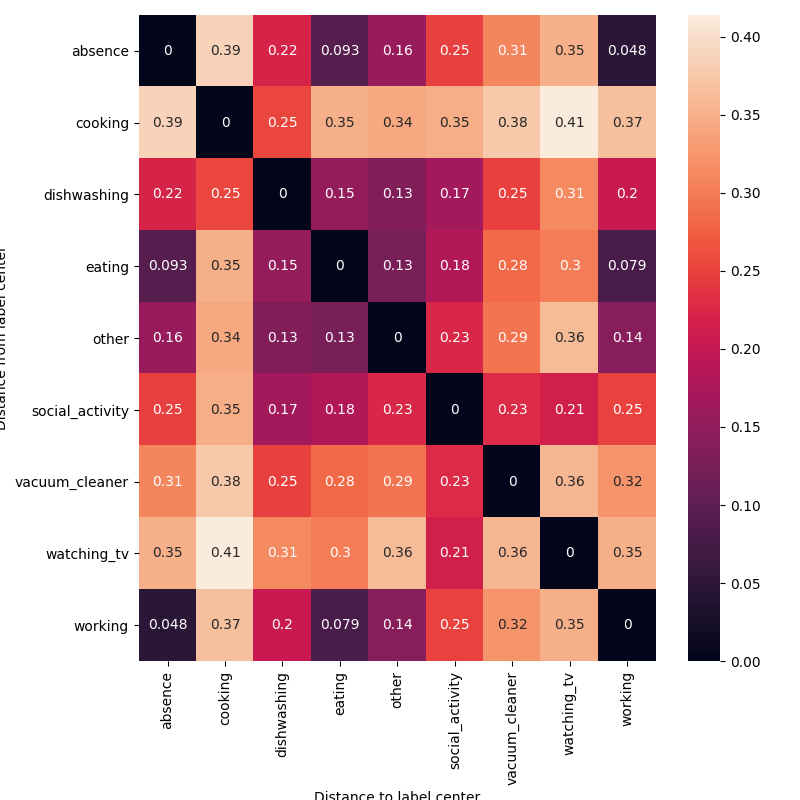
\includegraphics[width=0.5\linewidth]{study-doc/experiment_margin/assets/distance_mat_margin_1.png}
    \caption{Distance matrix of the margin=\texttt{1.0}}
    \label{fig:dist-margin-1}
\end{figure}
\noindent
One of the most important hyperparameter when training a triplet loss is the margin, which is denoted as $\alpha$. The margin makes sure that the network is not allowed to output the trivial solution, where all the embedding vectors are zero or contain the same values. In the triplet loss function, $\alpha$ is used to put a limit on how far the network can push the negative sample away to improve the loss. Thus the distance of the negative sample has to be higher than the distance from the anchor to the positive sample plus the margin $\alpha$. This experiment aims to show the importance of the margin as well as desires to find the optimal margin for the \gls{DCASE} dataset. The margin is evaluated for six different values \texttt{[0.3, 0.5, 0.7, 1, 2, 10]}.
\newline
\newline
The experiment was conducted by training five models with the same hyperparameters for ten epochs. To evaluate the optimal value for $\alpha$, the value of the triplet loss is used, since it has the most significant impact on it. The resulting embeddings improved from the trivial solution as the margin is increased. When the margin is decreased the total number of triplets generated whose loss is higher than zero decreases, therefore, they do not contribute to the training of the model and therefore reduce the performance of the model.
\newline
\newline
The highest and lowest margin can be omitted simply by examining the triplet loss because the lowest margin does not contribute to the training and the highest sets a constraint which can only be satisfied by a small number of triplets. To choose between the other margins is a much harder decision since the loss value is fairly the same. However, when looking at the resulting embedding space, it can be seen that the model using the \texttt{margin=1.0} results in a space, where the distances between the centroids of each label are fairly equally distributed. This characteristic of the embedding space is the one striving for. Figure \ref{fig:dist-margin-1} shows the distance matrix of the \texttt{margin=1.0}. When examining the embedding spaces from the other margins, it is observed that they do not have such an equally distributed distance matrix. Therefore the \texttt{margin=1.0} is chosen as the optimal parameter for the \gls{DCASE} dataset and is used in all of the further experiments as a hyperparameter.

\subsection{Experiment: segment size}
\label{sub:Experiment-Segment-Size}
\begin{figure}[hb]
\centering
    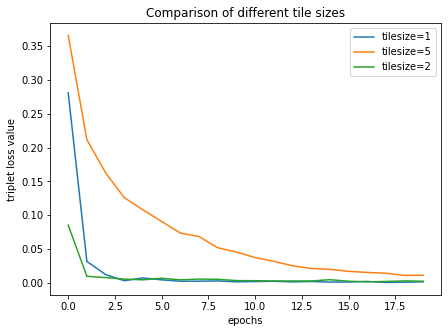
\includegraphics[width=0.5\linewidth]{study-doc/experiment_tile_size/assets/tile_sizes_plot.png}
    \caption{Plot of the triplet loss of the different segment sizes}
    \label{fig:tile-size-plot}
\end{figure}
\noindent
The size of each triplet, which is fed to the network, is an essential hyperparameter which needs to be carefully chosen. Because it specifies how much information each segment contains and is therefore fed to the network. If the segments are chosen too small, it does not contain enough information to distinguish between categories. If the size is too big, the segment contains too much information, and therefore, the model needs to work with a lot more data and gets a lot heavier. This experiment is conducted to find an optimal segment size for the triplets. The sample segment size is evaluated for three different values \texttt{[1, 2, 4]} in seconds.
\newline
\newline
The experiment was conducted by training three models with the same hyperparameters for 20 epochs. As a primary evaluation criterion for comparing the different segment sizes, the triplet loss is used, since the size mostly affects this value, because it should show how much of an audio sample is needed to distinguish between the different classes. Figure \ref{fig:tile-size-plot} shows all the trained models in a single plot to visualise the impact of changing the sample size. However, it is quite hard to interpret the different graphs since all of them are nearly zero or become zero very swiftly.
\newline
\newline
The figure \ref{fig:tile-size-plot} shows that the segment size 5s has the highest loss value, while the segment sizes 1s and 2s have relatively similar values. However, this does not mean that the segment size of 5s is the worst out of the three, it instead means that the model finds it harder to distinguish audio files when a larger sample is available, which is pretty evident since longer samples contain more information. Further, the figure \ref{fig:tile-size-plot} shows that the segment sizes of 1s and 2s have a very steep graph at the beginning and then hardly change their value. This indicates that it is relatively simple to achieve a good loss value with small audio samples, which means that the model can easily distinguish between small samples. This is as well reasonable since smaller segments contain a lot less information, and therefore, it is easier to distinguish between then since there is not enough information. Figure \ref{fig:tile-size-experiment-embedding-space} shows the embedding space visualised using the Embedding Projector from the Tensorboard, which visualises the space by computing a \gls{PCA} with three dimensions. This figure shows that the embedding space using a segment size of 5s (\ref{fig:embedding-5s}) results in much clearer clusters than when using 1s segments (\ref{fig:embedding-1s}). 
\newline
\newline
If the optimal parameter for the segment size would only be chosen from the loss value and therefore, from the plot \ref{fig:tile-size-plot}, it would be quite hard. However, since the visualisation of the embedding space shows a clear benefit in using a larger size, the segment size of 5s is chosen to be the optimal one for the \gls{DCASE} dataset. This can be explained because smaller samples much often contain sounds which do not indicate a specific sound in that class, say for example there is a two-second silence in a sound file of the class eating, it would be projected in the nearby region of silence in a sound of a different class, which is useful for other applications but since the goal is to achieve a best possible embedding space, this is not a satisfying result. Therefore, the larger sound segments are more robust to such problems, since they hold much more information about the resulting classes. 
\newline
\newline
If the thesis focused on supervised triplet loss, it would make sense to cut the audio files in much smaller segments than in the unsupervised setting, since in supervised learning the triplet selection makes sure that the clustering focuses on the classes and not some other arbitrary criteria, which happens in unsupervised learning. In the unsupervised triplet loss, it is challenging to examine what exactly is being clustered, because there can be an underlying structure which can not be seen for us humans.
\begin{figure}[htb]
\centering
\begin{subfigure}{.5\linewidth}
  \centering
  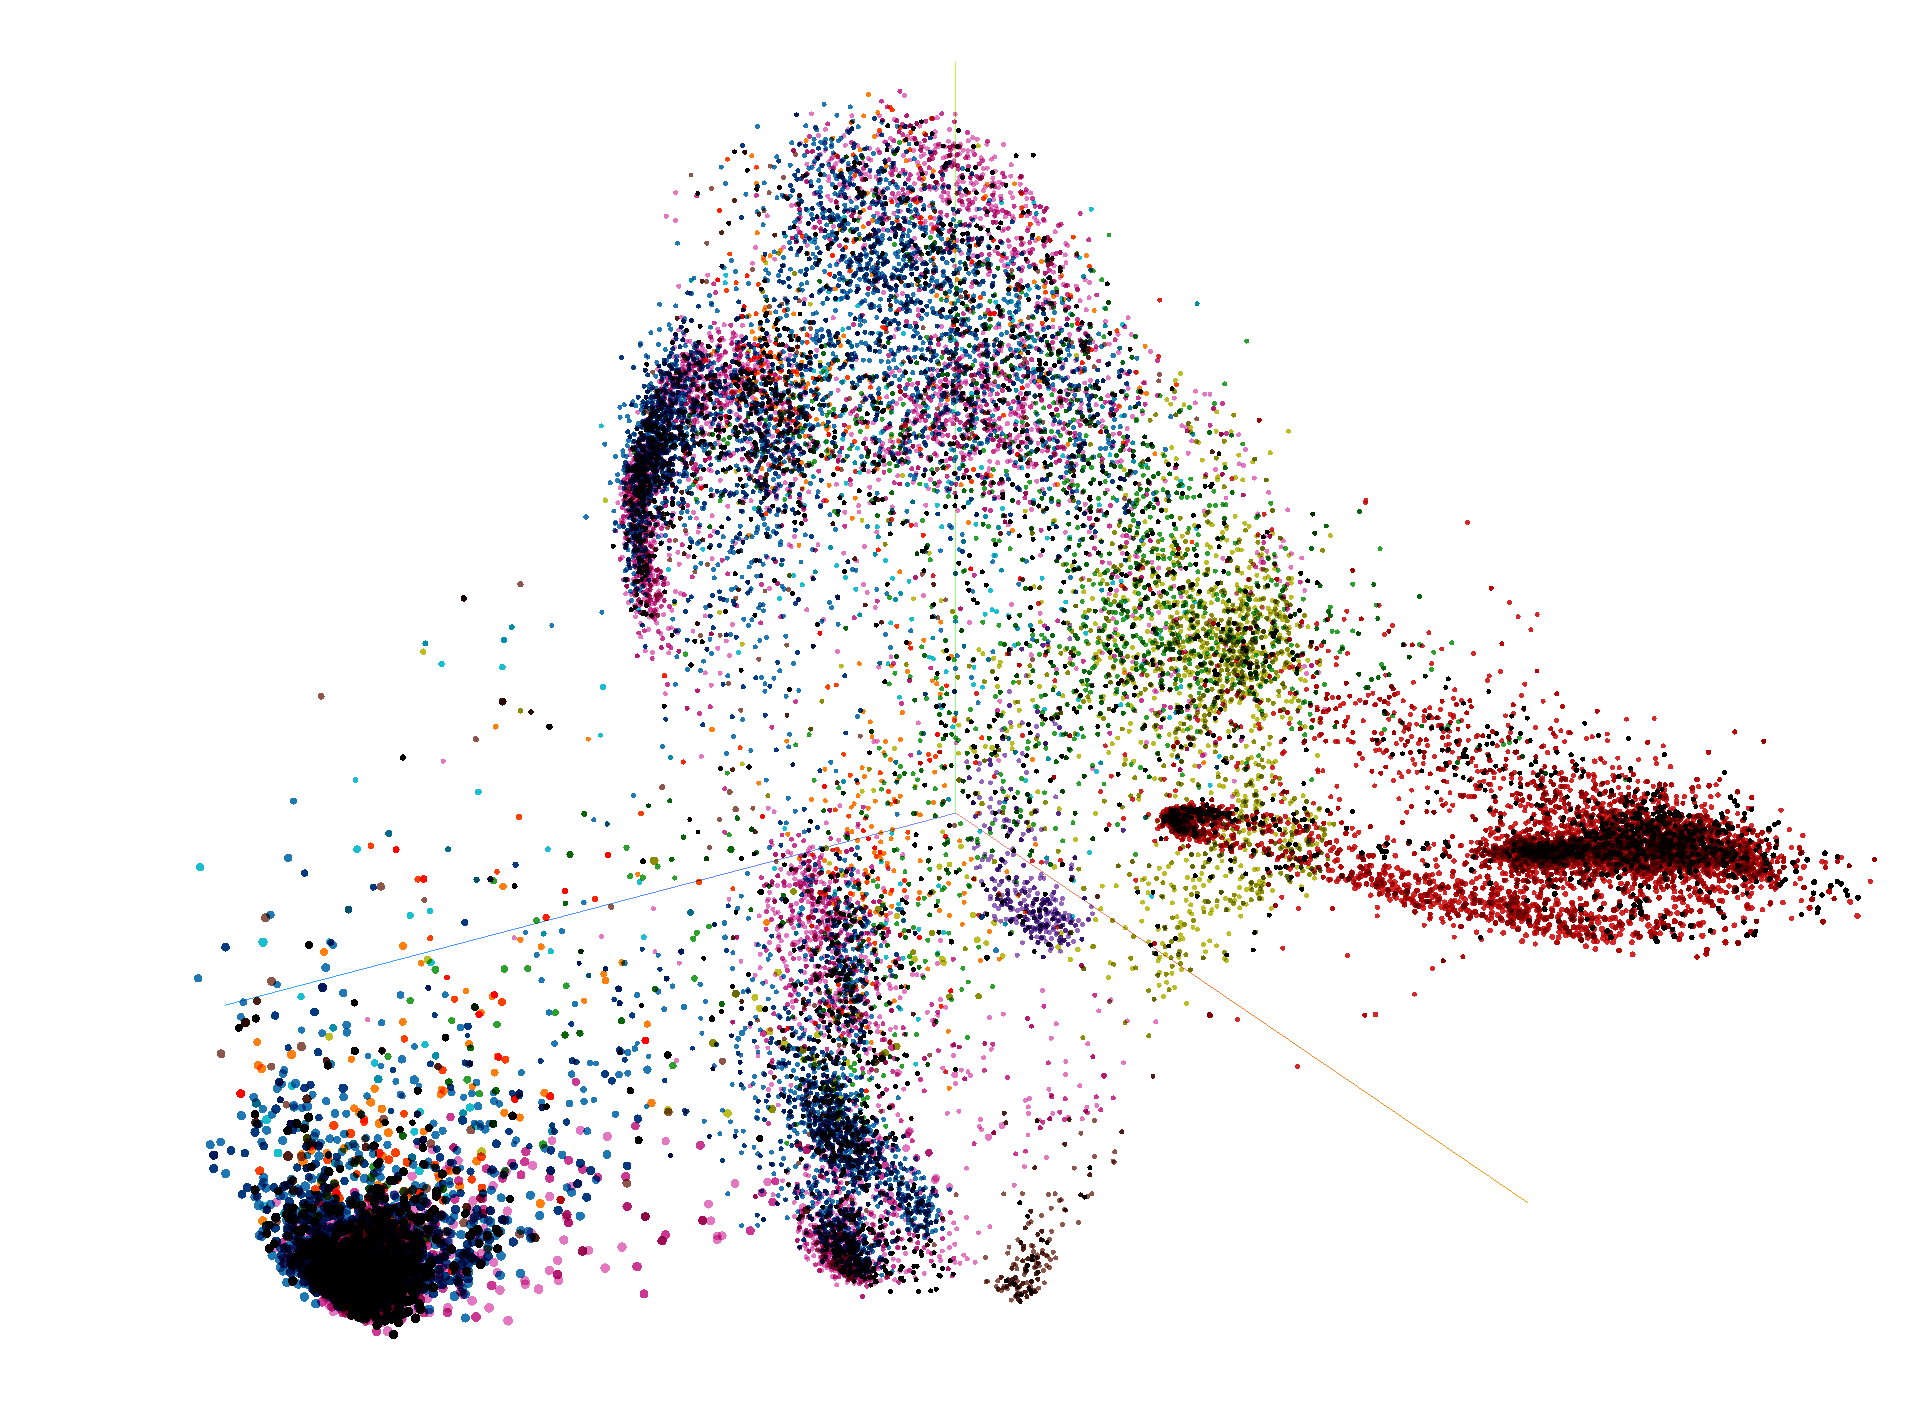
\includegraphics[width=.6\linewidth]{study-doc/experiment_tile_size/assets/embedding_space_5s.png}
  \caption{segment size 5s}
  \label{fig:embedding-5s}
\end{subfigure}%
\begin{subfigure}{.5\linewidth}
  \centering
  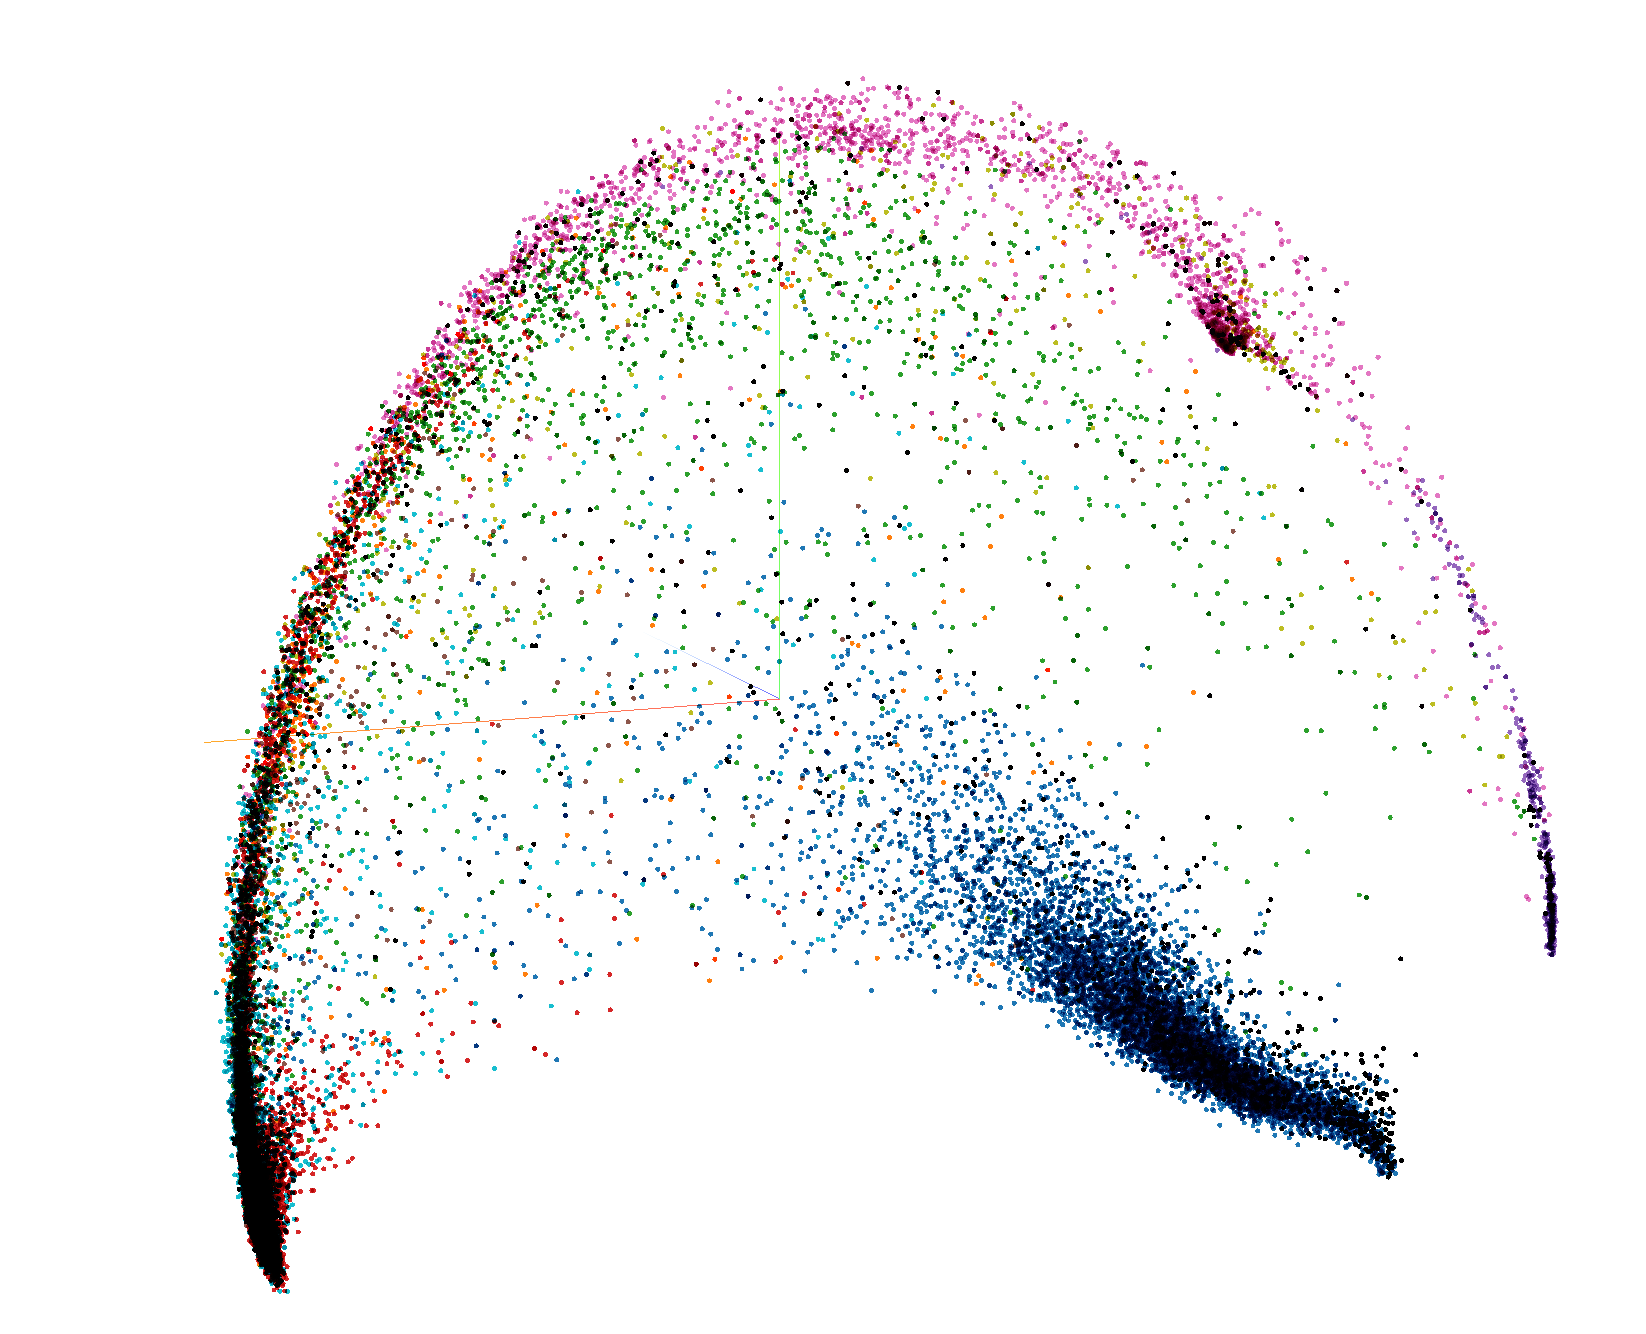
\includegraphics[width=.6\linewidth]{study-doc/experiment_tile_size/assets/embedding_space_1s.png}
  \caption{segment size 1s}
  \label{fig:embedding-1s}
\end{subfigure}
\caption{Visualisation of the embedding space from the segment size 5s and 1s}
\label{fig:tile-size-experiment-embedding-space}
\end{figure}

\subsection{Experiment: embedding size}
\label{sub:Experiment-Embedding-Size}
\begin{figure}[htb]
\centering
    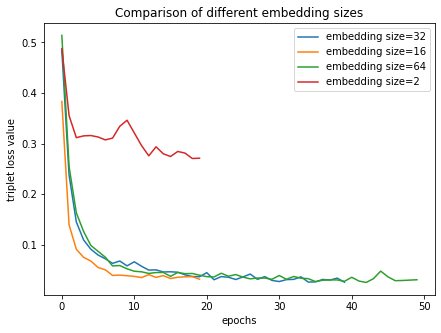
\includegraphics[width=0.5\linewidth]{study-doc/experiment_embedding_size/assets/plot_embedding_sizes.png}
    \caption{Plot of the triplet loss of the different embedding sizes}
    \label{fig:plot-embeddings-epochs}
\end{figure}
\noindent
The experiment aims to show the effect of the size of the last dense layer from the embedding architecture, further called the embedding size. The size of the embedding space is essential for the performance, since choosing the wrong hyperparameter can lead to over- or underfitting of the model. The size defines how many dimensions the resulting embedding space has. Therefore if this parameter $e$ is selected to be too big, the model almost certainly overfits, because the model has many options to project the input data onto the embedding space. However, if $e$ is chosen to be too small, there is not enough room to project inputs in different regions. This experiment aims to search an optimal parameter for $e$. The embedding size $e$ is evaluated for four different values \texttt{[2, 16, 32, 64]}.
\newline
\newline
The experiment was conducted by training four models with the same hyperparameters for a different amount epochs. The training was stopped when no more learning was observed. Since comparing the different embedding sizes is pretty hard because most of the metrics in the thesis focus on distances between embedding points. In higher dimensional embedding spaces, distances have a different scale and different meanings. This is especially true if small embedding sizes, such as \texttt{2}, and large sizes, such as \texttt{64}, are compared with each other. Therefore a simple classifier was trained on the resulting embedding spaces, and the metrics of the classifier was compared to find the optimal parameter. To further compare the embedding spaces, they were visualised using the Tensorboard Embedding Projector and manually compared with each other.
\newline
\newline
The figure \ref{fig:plot-embeddings-epochs} shows the different triplet loss values of the embedding sizes. The embedding size \texttt{2} has a significantly higher value than the other embedding sizes, which shows that in the two-dimensional embedding space, it is a lot harder to project the data points apart from each other. Whereas in high dimensional embedding spaces, the model can easier build clusters.
\begin{figure}[t]
\centering
\begin{subfigure}{.33\linewidth}
  \centering
  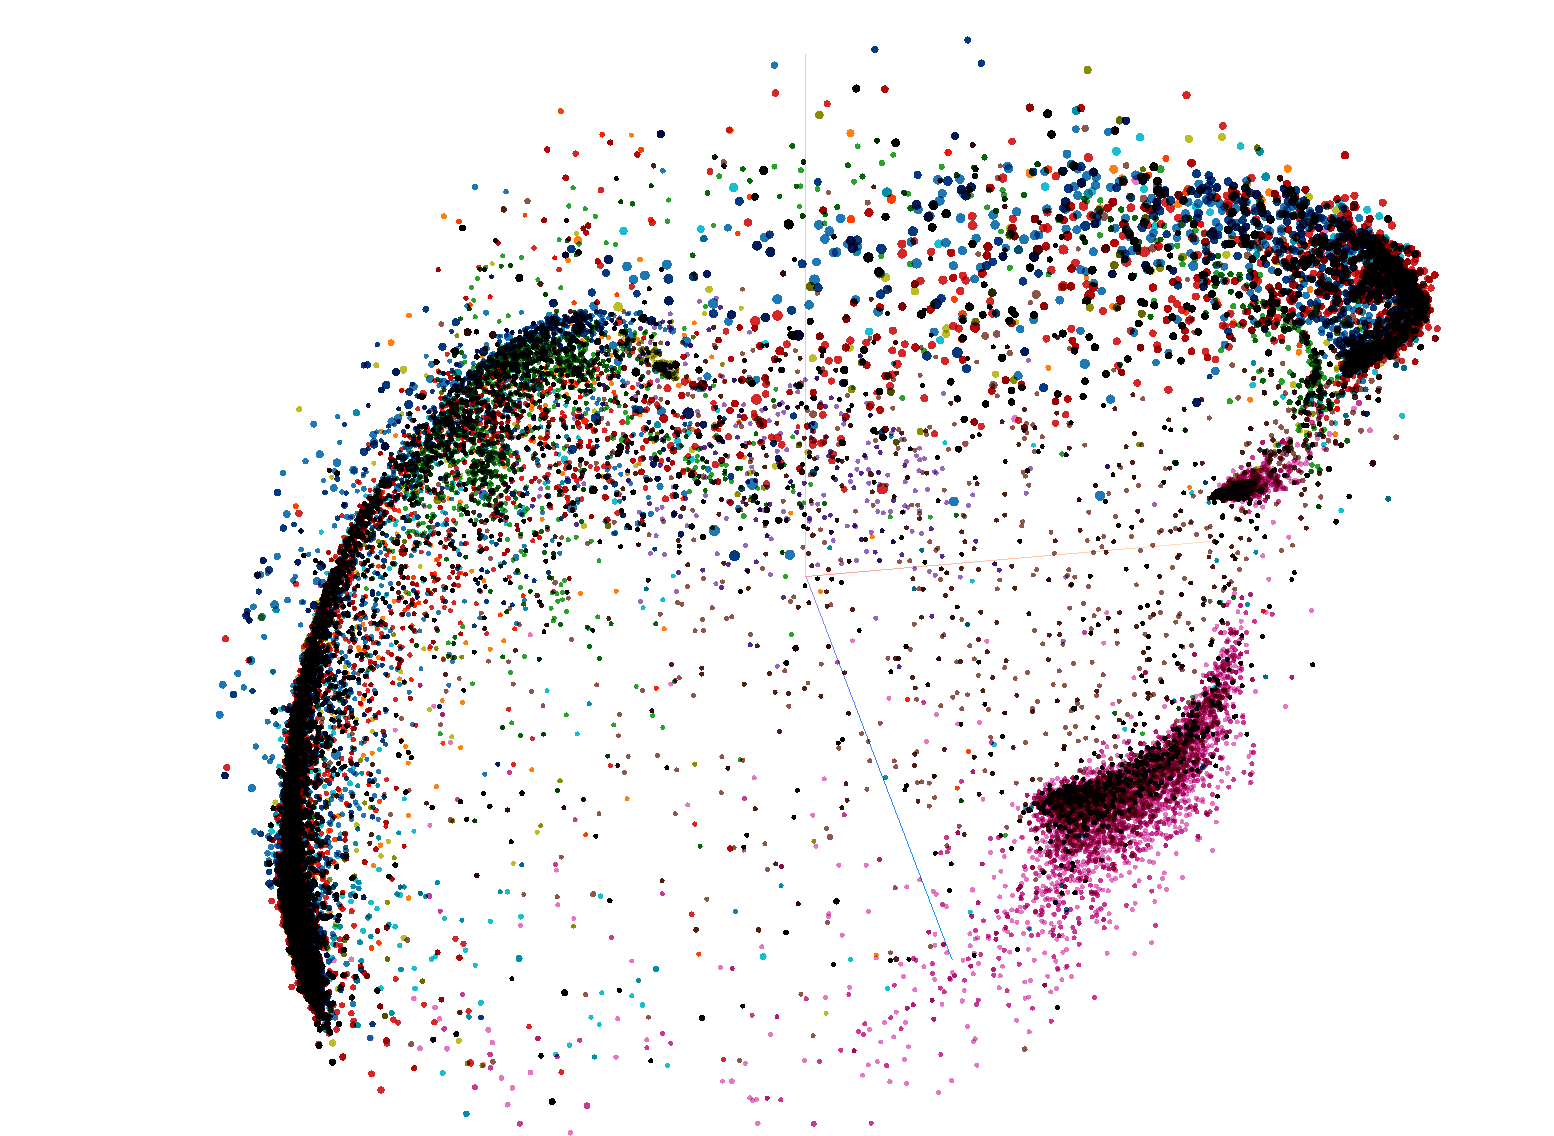
\includegraphics[width=.9\linewidth]{study-doc/experiment_embedding_size/assets/embedding_space_16.png}
  \caption{embedding size 16}
  \label{fig:embedding-space-16}
\end{subfigure}%
\begin{subfigure}{.33\linewidth}
  \centering
  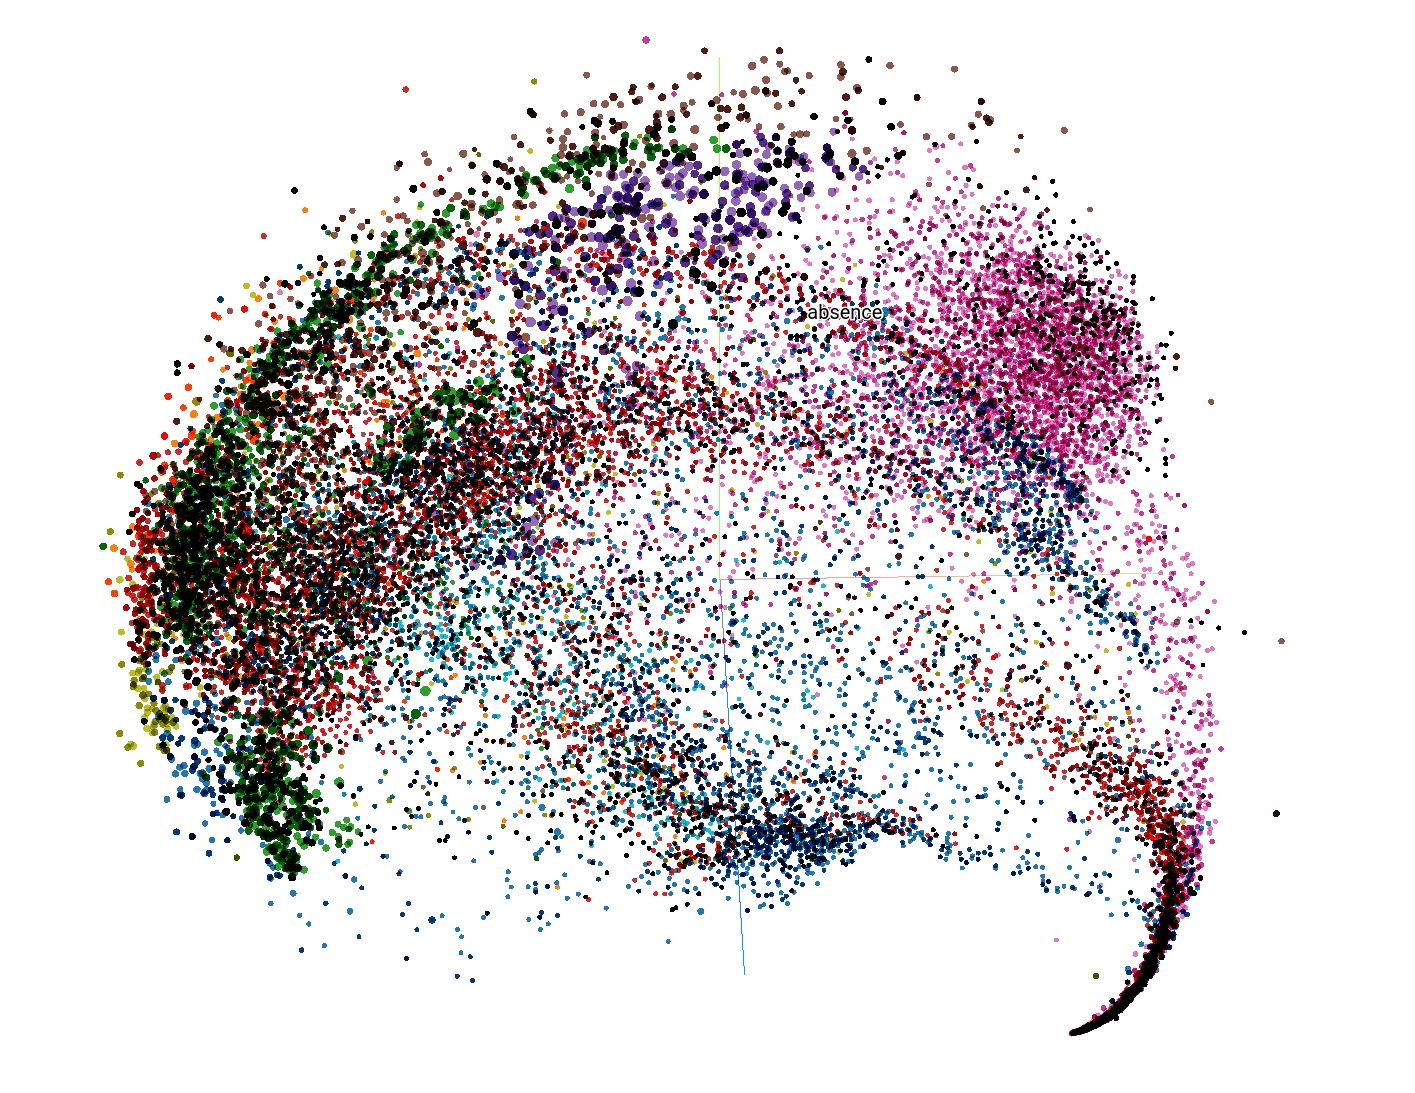
\includegraphics[width=.9\linewidth]{study-doc/experiment_embedding_size/assets/embedding_space_32.png}
  \caption{embedding size 32}
  \label{fig:embedding-space-32}
\end{subfigure}%
\begin{subfigure}{.33\linewidth}
  \centering
  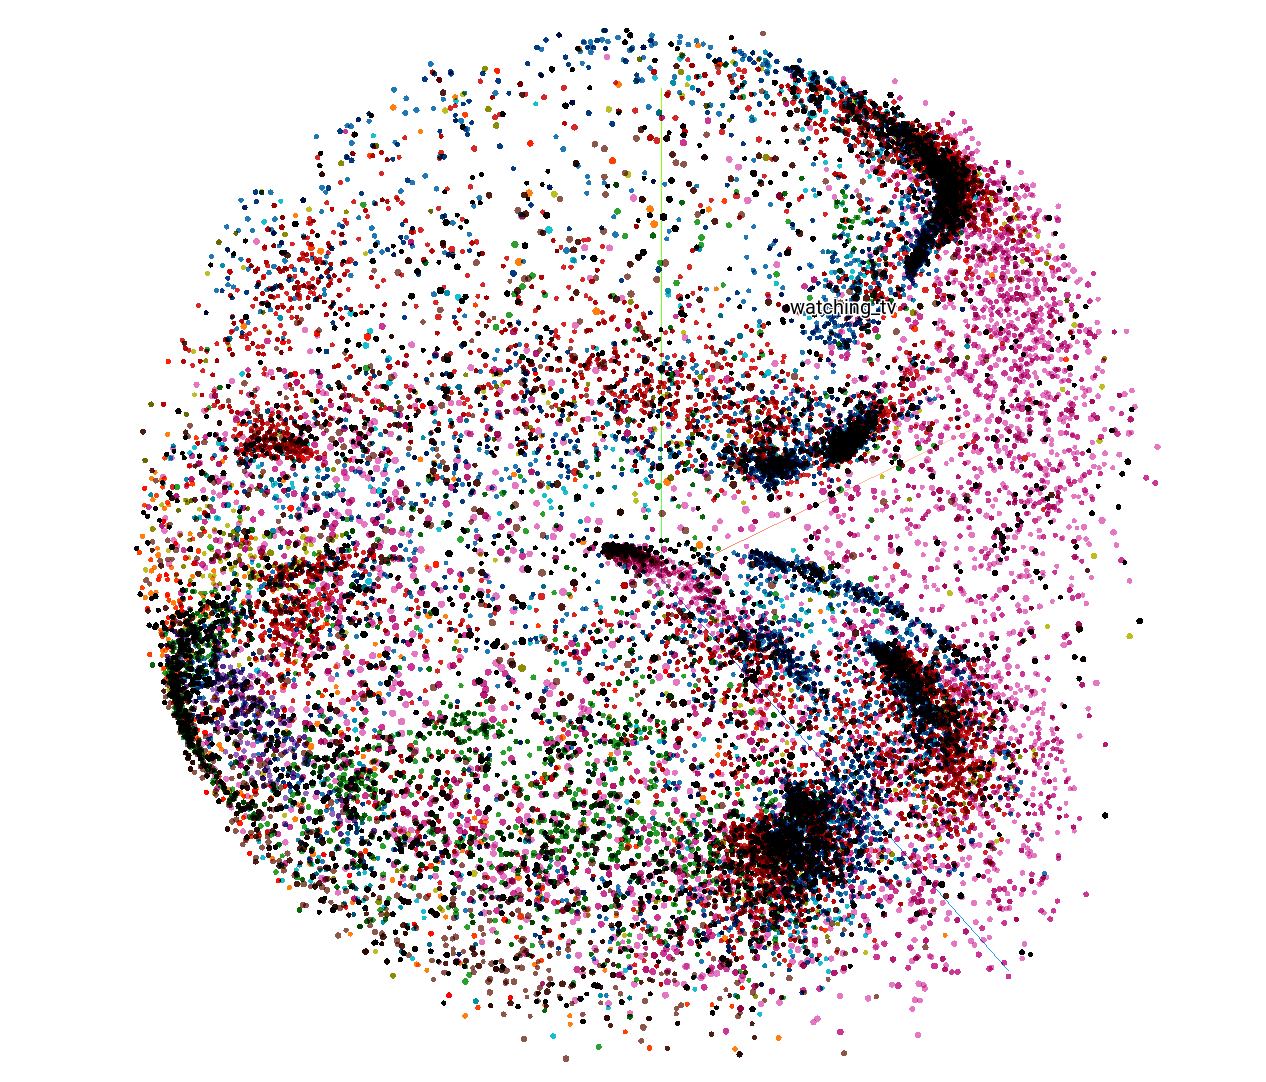
\includegraphics[width=.9\linewidth]{study-doc/experiment_embedding_size/assets/embedding_space_64.png}
  \caption{embedding size 64}
  \label{fig:embedding-space-64}
\end{subfigure}
\caption{Plot of the resulting embedding spaces}
\label{fig:embedding-size-experiment-embedding-space}
\end{figure}
\newline
\newline
\noindent
The plot further shows that the loss value of the embedding sizes \texttt{16, 32, 64} are relatively similar and are therefore further compared by examining their resulting embedding space. Which is shown in figure \ref{fig:embedding-space-16}, \ref{fig:embedding-space-32} and \ref{fig:embedding-space-64}. The result shows that there are vast differences in the embedding spaces, even though the triplet loss value is not that different. The embedding size of \texttt{16} shows only approximately four resulting clusters, which indicates a noisy embedding space where small classes are not well separated from each other. The embedding space of \texttt{32} and \texttt{64} show significant more resulting clusters and they result therefore in a better embedding space. However, it is to say that both embedding spaces further have more noise in it than the lower-dimensional space.
\newline
\newline
The graph \ref{fig:embedding-size-classifier-f1} shows the resulting F1 score when a simple logistic classifier is trained on top of the resulting embedding space. Since the \gls{DCASE} dataset is heavily unbalanced, the F1 score is compared. All of the classifiers are trained for 20 epochs using the same parameters as the one for training the embedding space. The figure \ref{fig:embedding-size-classifier-f1} shows that the F1 score of the embedding space, where \texttt{16} accomplished the highest out of the three. The graph \ref{fig:embedding-size-classifier-loss} shows the corresponding sparse categorical cross-entropy loss value of the classifier trained on the embedding spaces \texttt{16} and \texttt{64}.
\newline
\newline
The figure \ref{fig:plot-embeddings-epochs} shows that the smallest embedding size can be omitted since it has the highest triplet loss value significantly. The other three embedding spaces have quite similar values and are, therefore, further compared. The trained classifier on top of the embedding space shows (figure \ref{fig:embedding-size-classifier-f1}) that the embedding size \texttt{32} can be omitted since it has a significantly lower score than the others. The figure \ref{fig:embedding-size-classifier-f1} shows, that the embedding size \texttt{16} has achieved the highest F1 score of approximately \texttt{0.39}. However, the figure \ref{fig:embedding-size-classifier-loss} shows that the loss value of the embedding size \texttt{16} converges, which indicates that the training process is finished and the classifier will not show any improvements when training longer. The embedding size \texttt{64} has a lower F1 score, but the loss value is still decreasing at the end of epoch 20, which indicates that the model can benefit from further training. Further training will increase the F1 score until it converges.
\begin{figure}[t]
\centering
\begin{subfigure}{.5\linewidth}
  \centering
  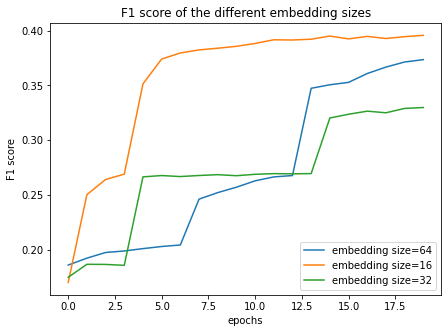
\includegraphics[width=.9\linewidth]{study-doc/experiment_embedding_size/assets/classifier_f1.png}
  \caption{F1 score}
  \label{fig:embedding-size-classifier-f1}
\end{subfigure}%
\begin{subfigure}{.5\linewidth}
  \centering
  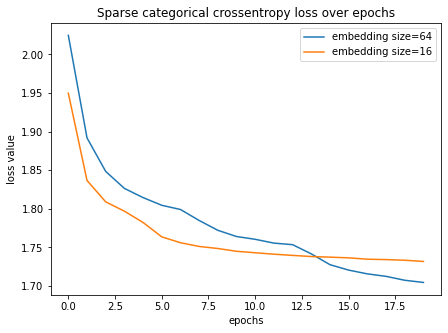
\includegraphics[width=.9\linewidth]{study-doc/experiment_embedding_size/assets/classifier_loss.png}
  \caption{sparse categorical cross-entropy loss}
  \label{fig:embedding-size-classifier-loss}
\end{subfigure}
\caption{graph of the metrics from the different classifiers trained on top of the resulting embedding spaces}
\label{fig:embedding-size-experiment-classifier-metrics}
\end{figure}
\newline
\newline
\noindent
Because of this result, the optimal embedding size, out of the four, is \texttt{64}, since it has an optimal triplet loss value, a high enough F1 score and the loss value still decreases after 20 epochs of training the classifier. For the next experiments, the embedding space size \texttt{64} is chosen. The embedding space should also be evaluated on significant higher spaces, such as \texttt{256} or \texttt{512} (\ref{sub:Experiment-Larger-Embedding-Sizes}).
\newline
\newline
The experiment further showed, that the longer the embedding space was trained, the more the loss value oscillates which indicates that a learning rate decay should be used to reduce the learning rate over time (\ref{fig:plot-triplet-64}). It further showed, that the triplet loss value vanished after ten epochs of training (\ref{fig:plot-embeddings-epochs}, which indicates that the model fails to learn the underlying structure of the data. This can have many different reasons, one of the most plausible assumptions is, that the model overfits, because the model succeeds in learning representation of the data (\ref{fig:embedding-size-experiment-embedding-space}). However, when this particular representation is learnt, the model stops to train and only produces a low loss. To mitigate the problem of overfitting, an L2-normalisation will be implemented, and an experiment to find the optimal regularisation factors is conducted (\ref{sub:Experiment-Regularisation-Factor}).
\begin{figure}[htb]
\centering
    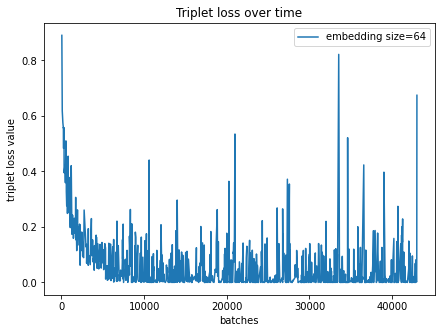
\includegraphics[width=0.4\linewidth]{study-doc/experiment_embedding_size/assets/plot_triplet_loss.png}
    \caption{Plot of the triplet loss of the embedding space 64}
    \label{fig:plot-triplet-64}
\end{figure}

\subsection{Experiment: regularisation factor}
\label{sub:Experiment-Regularisation-Factor}
\begin{figure}[H]
\centering
    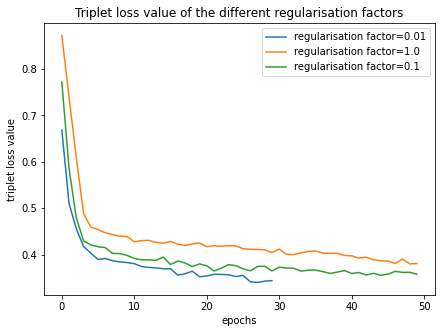
\includegraphics[width=0.5\linewidth]{study-doc/experiment_regularisation/assets/triplet_loss.png}
    \caption{Plot of the triplet loss values of the different regularisation factors $\lambda$}
    \label{fig:plot-triplet-loss}
\end{figure}
\noindent
The experiment aims to show how the embedding space will change for different regularisation factors. The purpose of regularisation is that it prevents models from overfitting, by penalising high weights. The regularisation is calculated for all layers weights separately and is then added to the standard loss function, in this case, the triplet loss. The combined loss value is then used to calculate the gradients and update the weights of the model. There are a lot of different regularisation techniques, which successfully reduce the chance of overfitting. In this experiment, the \texttt{L2-Regularisation} is used and evaluated with different values. The parameter which will control the value of the \texttt{L2-Regularisation} is denoted as $\lambda$. The regularisation factor $\lambda$ will be evaluated for three different values \texttt{[1.0, 0.1, 0.01]}.
\newline
\newline
To compare the different resulting embedding spaces, a simple logistic classifier is trained on top of the resulting embedding spaces, which aims to show how well a simple classifier works with the embedding space. This will show how good the resulting embedding space is. The classifier is trained for 20 epochs with the same parameters as the embedding model.
\newline
\newline
Figure \ref{fig:plot-triplet-loss} shows the difference between the triplet loss values of the embedding model when changing the regularisation factor. It shows that the model with $\lambda = 1.0$ has the highest triplet loss value, which is obvious, since the bigger the regularisation factor is, the longer the model optimises the weights to satisfy the constraint of having very small weights. The lower $\lambda$, the faster the model optimises the triplet loss value. $\lambda = 0.01$ has the lowest triplet loss value.
\begin{figure}[tb]
\centering
\begin{subfigure}{.5\linewidth}
  \centering
  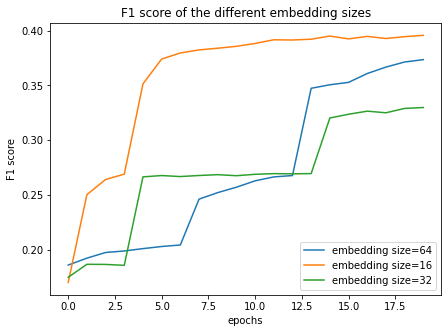
\includegraphics[width=.9\linewidth]{study-doc/experiment_embedding_size/assets/classifier_f1.png}
  \caption{F1 score}
  \label{fig:regularisation-experiment-classifier-f1}
\end{subfigure}%
\begin{subfigure}{.5\linewidth}
  \centering
  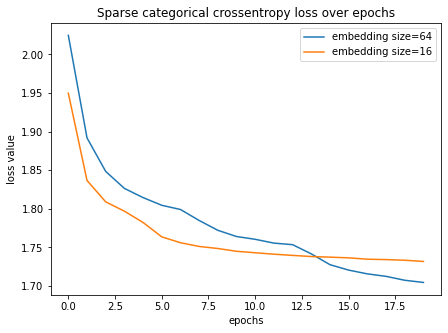
\includegraphics[width=.9\linewidth]{study-doc/experiment_embedding_size/assets/classifier_loss.png}
  \caption{sparse categorical cross-entropy loss}
  \label{fig:regularisation-experiment-classifier-loss}
\end{subfigure}
\caption{graph of the F1 score and the loss from the different classifiers trained on top of the resulting embedding spaces}
\label{fig:regularisation-experiment-classifier-metrics}
\end{figure}
\newline
\newline
\noindent
Figure \ref{fig:regularisation-experiment-classifier-f1} shows the different F1 scores of the logistic classifier, which is trained on top of the embedding architecture. This provides an idea of how well the embedding space separates the classes and therefore gives a performance gain. The figure \ref{fig:regularisation-experiment-classifier-f1} shows, that the regularisation factor $\lambda = 0.01$ has the highest F1 score. This result is significant since this particular embedding space was only trained for 30 epochs, unlike the other models, who are trained for 50. 
\newline
\newline
The figure \ref{fig:regularisation-experiment-classifier-loss} shows the corresponding categorical cross-entropy loss values of the trained classifiers. It shows that the loss of $\lambda = 1.0$ converges before $\lambda = 0.1$ or $\lambda = 0.01$. The figure further shows, that the loss values of $\lambda = 0.1$ and $\lambda = 0.01$ are not converged and would benefit from a longer training.
\newline
\newline
Figure \ref{fig:regularisation-experiment-classifier-f1} shows that the highest regularisation factor $\lambda = 1.0$ can be omitted since it did not accomplish an equally good F1 score. This result is expectable since a high regularisation factor forces the embedding model to work with very small weights and can, therefore, lead to performance loss. 
\newline
\newline
The regularisation factor $\lambda = 0.1$ and $\lambda = 0.01$ only show very little difference in F1 performance as well as in triplet loss value. Never the less, the factor $\lambda = 0.01$ provides slightly better results than $\lambda = 0.1$. The triplet loss value and the loss value of the classifier of the regularisation factor $\lambda = 0.01$ is still decreasing at the end of the training, which indicates that the model can benefit from further training. Further training will increase the resulting embedding space and the F1 score of the classifier until it converges.
\newline
\newline
The figure \ref{fig:plot-triplet-loss} and \ref{fig:regularisation-experiment-classifier-f1} further indicate one essential conclusion, that the value of the triplet loss is directly related to how well the classifier performs, which is further an indication how well the created embedding space works. Therefore the assumption is, that the lower the triplet loss value, the better the classifier performs and the better the embedding space is. 
\newline
\newline
The experiment shows that the regularisation factor $\lambda = 0.01$ gives the best results out of the three since it has an optimal triplet loss value, a high enough F1 score and the loss value still decreases after 20 epochs of training the classifier. The experiment showed that the regularisation factor $\lambda$ has an essential impact on the embedding space and should therefore not be chosen to be too big nor too small since this either leads to over- or underfitting.

\subsection{Experiment: feature representation}
\label{sub:Experiment-Feature-Representation}
\begin{figure}[htb]
\centering
\begin{subfigure}{.5\linewidth}
  \centering
  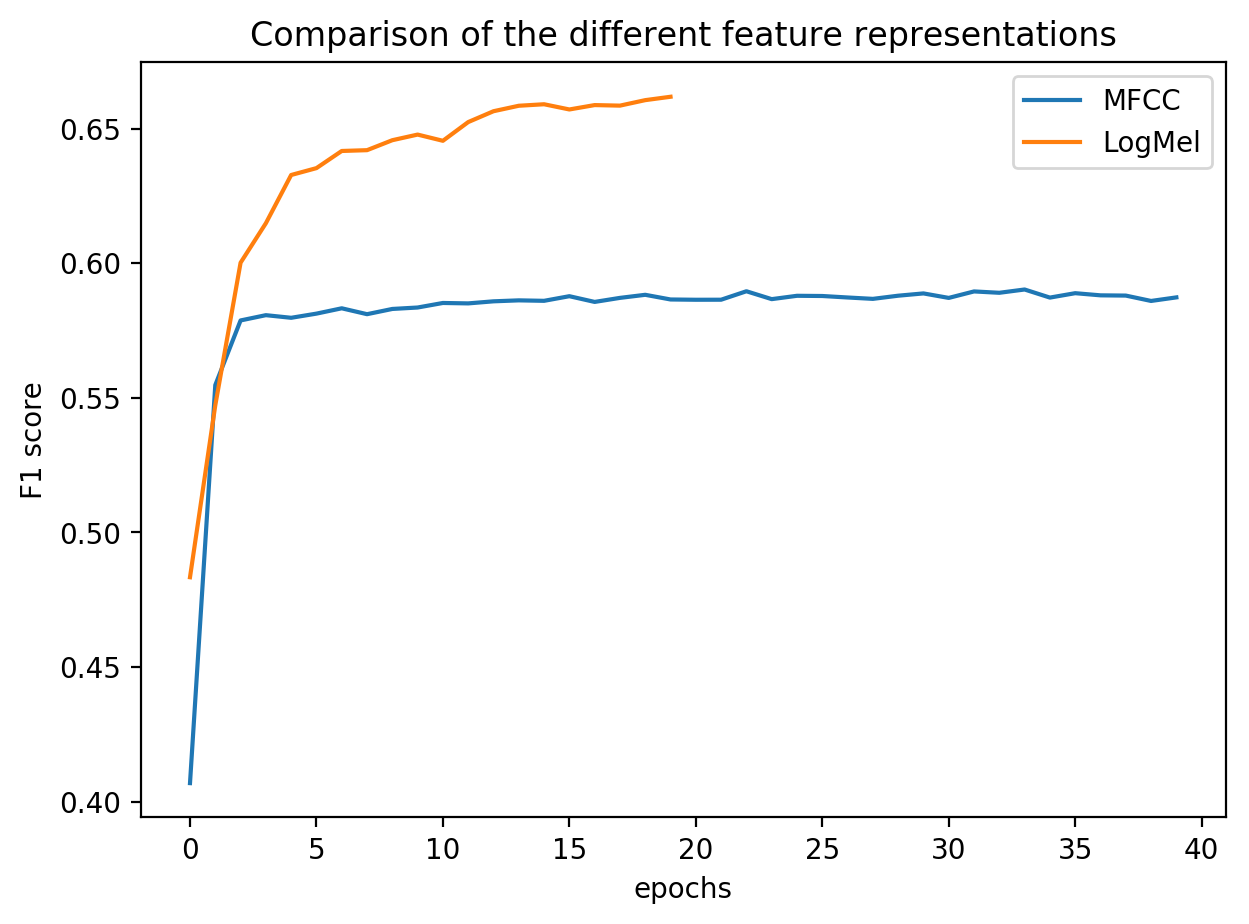
\includegraphics[width=.9\linewidth]{study-doc/experiment_feature/assets/f1_feature_representation.png}
  \caption{Triplet loss}
  \label{fig:plot-triplet-loss-feature-representations}
\end{subfigure}%
\begin{subfigure}{.5\linewidth}
  \centering
  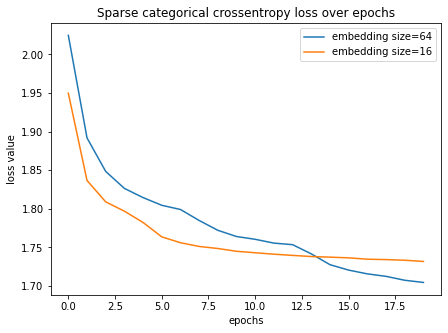
\includegraphics[width=.9\linewidth]{study-doc/experiment_embedding_size/assets/classifier_loss.png}
  \caption{F1 score of the classifier}
  \label{fig:classifier-f1-feature-represenations}
\end{subfigure}
\caption{Plot of the metrics from the models trained using the different feature representations}
\label{fig:feature-experiment-metrics}
\end{figure}
\noindent
The purpose of the feature representation is to represent the audio in a more compact form than the raw audio. The feature representation further determines the input size for the model. There are a lot of different ways to represent an audio file in a more compact form. One of the most popular representations is \glspl{MFCC}, which is heavily used in the audio domain. However, in recent years, the trend leads more towards using the log Mel spectrogram, which is very similar to the \glspl{MFCC}, but by omitting the last step of the calculation. This experiment aims to find the optimal feature representation for the thesis. The optimal feature representation will be evaluated for \texttt{[LogMel, MFCCs]}.
\newline
\newline
To compare the different resulting embedding spaces, a simple logistic classifier is trained on top of the resulting embedding spaces, which aims to show how well a simple classifier works with the embedding space. This will show how good the resulting embedding space is. The classifier is trained for 40 epochs with the same parameters as the embedding model.
\newline
\newline
Figure \ref{fig:plot-triplet-loss-feature-representations} shows the difference between the triplet loss from the model using the different feature representations. It shows that the model trained using the \glspl{MFCC} results in a significantly lower loss than the model using the log Mel spectrogram. The model using the log Mel spectrogram seem already converging at epoch 30.
\newline
\newline
Figure \ref{fig:classifier-f1-feature-represenations} shows both of the F1 scores of the logistic classifier, which were trained using the embedding space as input. This provides an idea of how well the embedding space separates the classes and therefore gives a performance gain. The figure \ref{fig:classifier-f1-feature-represenations} shows clearly that the classifier trained on top of the log Mel spectrogram reached a higher F1 score than the \glspl{MFCC}. The metric further shows, that the classifier using the \glspl{MFCC} embedding space fails to improve the F1 score over time, whereas the classifier for the log Mel spectrogram shows a definite increase over time.
\newline
\newline
From figure \ref{fig:plot-triplet-loss-feature-representations} it seems that the optimal feature representation is the \glspl{MFCC} since it reached a significantly lower loss value. It further shows that the model would be able to benefit from further training since the model is still decreasing. However, when looking at the resulting F1 score of the classifiers (figure \ref{fig:classifier-f1-feature-represenations}), the result shows, that even though the \glspl{MFCC} representation reached a lower triplet loss, the classifier fails to separate the resulting clusters using a hyperplane. 
\newline
\newline
This experiment shows that the optimal feature representation for the current thesis is using the log Mel spectrogram, since it resulted in a higher F1 score of the classifier, even though the triplet loss value is higher than the one using the \glspl{MFCC}. This is mainly due to the different nature of the feature representations. The \glspl{MFCC} representation input size (498, 13) is significantly lower than the log Mel spectrogram representation input size (498, 128). The \glspl{MFCC} is a more compact representation, which seems to have a negative effect on the models' performance. This experiment shows that the model benefits from using a representation which has more features and therefore, the log Mel spectrogram is used as the optimal representation for the thesis.

\subsection{Experiment: larger embedding sizes}
\label{sub:Experiment-Larger-Embedding-Sizes}
\begin{figure}[htb]
\centering
\begin{subfigure}{.5\linewidth}
  \centering
  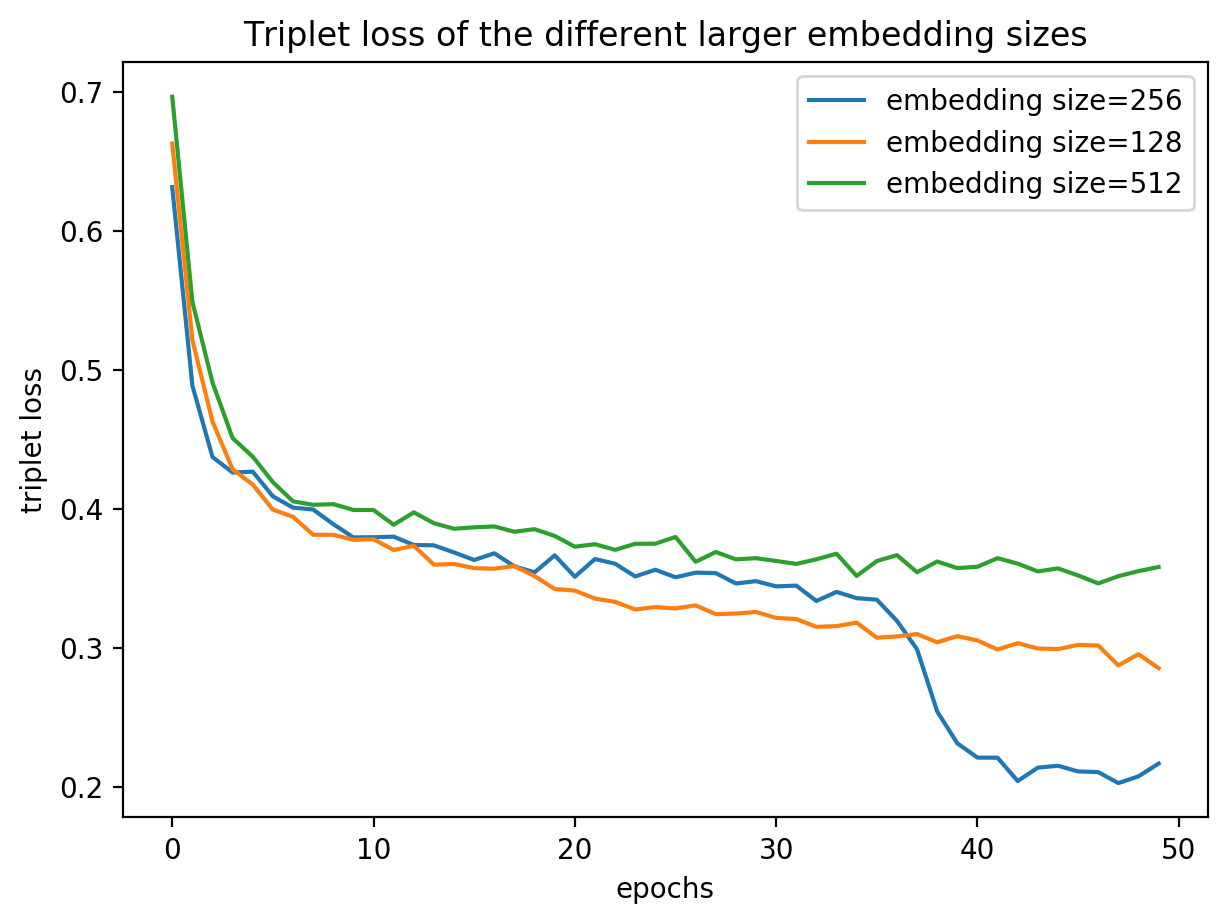
\includegraphics[width=.9\linewidth]{img/triplet_loss_dcase_embedding_large.png}
  \caption{Triplet loss}
  \label{fig:plot-triplet-loss-embedding-sizes-larger}
\end{subfigure}%
\begin{subfigure}{.5\linewidth}
  \centering
  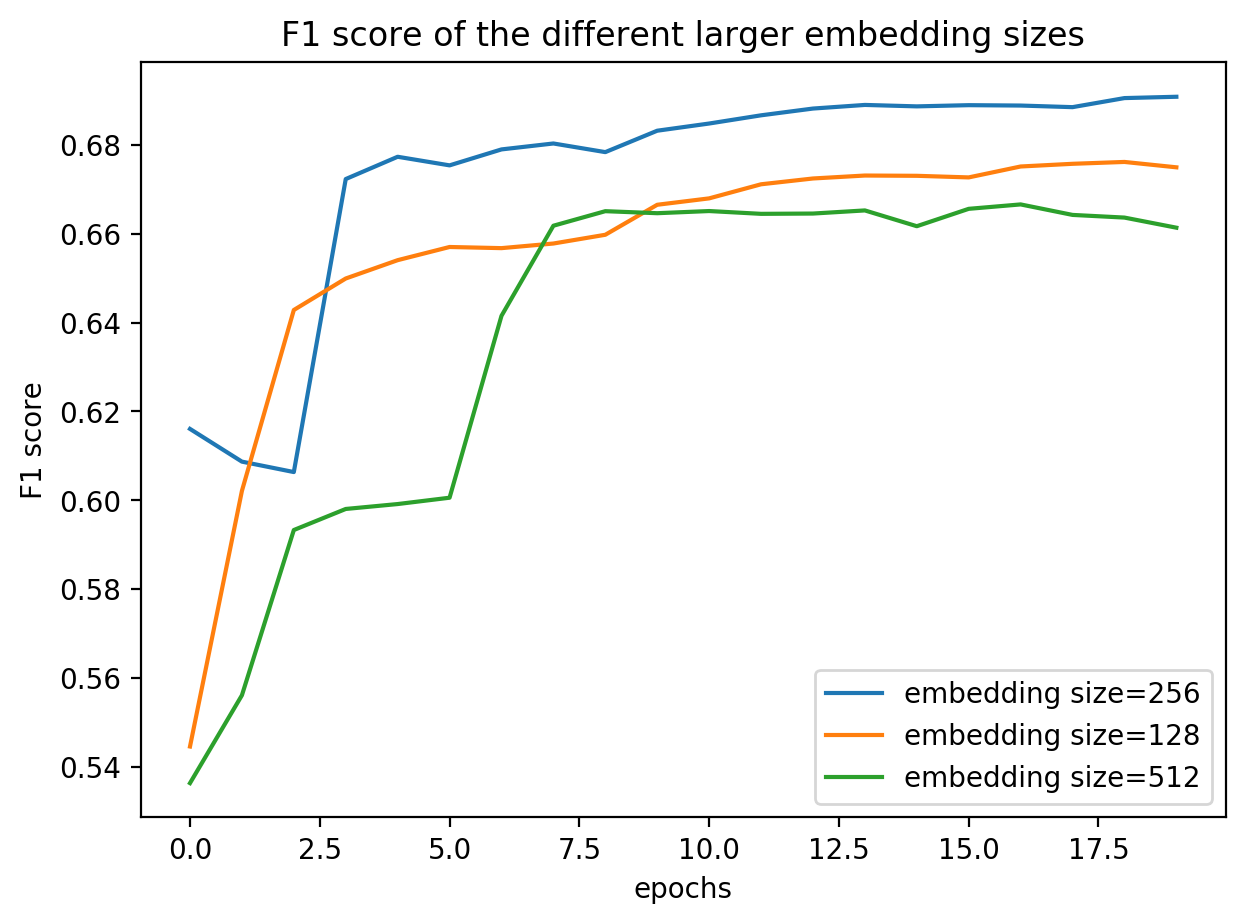
\includegraphics[width=.9\linewidth]{img/f1_dcase_embedding_large.png}
  \caption{F1 score of the classifier}
  \label{fig:classifier-f1-embedding-sizes-larger}
\end{subfigure}
\caption{Plot of the metrics from the models trained using the different larger embedding sizes}
\label{fig:embedding-sizes-larger-experiment-metrics}
\end{figure}
\noindent
The size of the embedding space $e$ is one of the most important hyperparameters in this thesis because it defines how big the size of the embedding space is. In the first part of finding the optimal size $e$, sizes \texttt{[2, 16, 32, 64]} were evaluated. The optimal embedding size was chosen to be \texttt{64} since it provided an optimal loss value and a high F1 score. To make sure that the optimal embedding size will be found, the same experiment was conducted again with larger embedding sizes and the improvements from the experiments conducted until now. Therefore the experiment is conducted again and evaluated for the embedding sizes  \texttt{[64, 128, 256]}. All of the models were trained for 50 epochs, since the experiments conducted before, showed that the models would still benefit from further training after epoch 30. The models were compared using the triplet loss value and the F1 score of the classifier, trained using the embedding space.
\newline
\newline
Figure \ref{fig:plot-triplet-loss-embedding-sizes-larger} shows the triplet loss graphs of the models trained with different embedding sizes. It shows that the embedding size \texttt{256} reached the lowest triplet loss value out of the three. Further, it shows that the embedding size \texttt{256} has decreased a significant amount between epoch 35 and 40, whereas the other models stayed around the same value. Figure \ref{fig:classifier-f1-embedding-sizes-larger} shows the macro-averaged F1 score of the different classifiers trained on top of the embedding space. The figure shows that the embedding size \texttt{256} reached the highest score of approximately 68\%.
\newline
\newline
From the figures \ref{fig:embedding-sizes-larger-experiment-metrics} it can be seen that the optimal embeddings size is \texttt{256} since it has clearly reached the lowest triplet loss and reached the highest F1 score out of the three sizes. Therefore, the embedding size \texttt{256} was chosen to be the optimal hyperparameter for the thesis.

\subsection{Triplet loss}
\label{sub:Results-Triplet-Loss}
\begin{figure}[htb]
\centering
    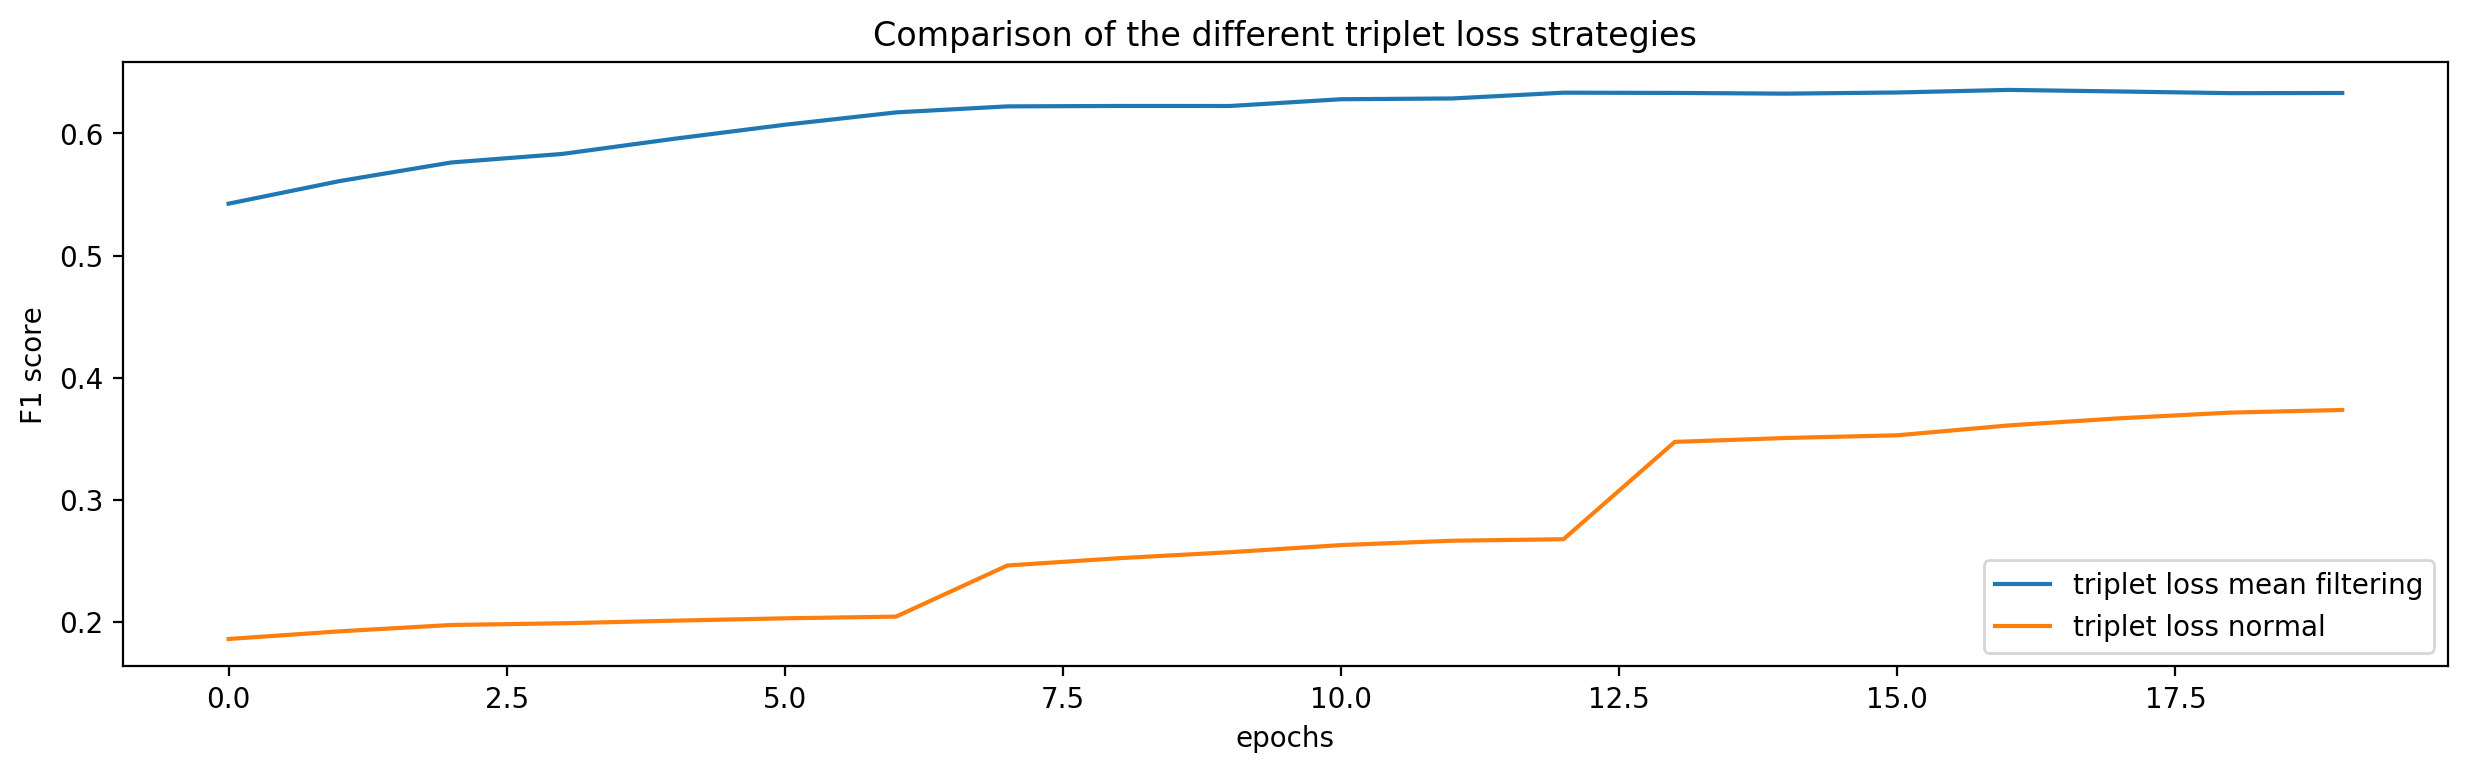
\includegraphics[width=0.6\linewidth]{img/Triplet-Loss-Comparison-Techniques.png}
    \caption{Triplet loss comparison of different techniques}
    \label{fig:Triplet-Loss-Techniques}
\end{figure}
\noindent
The first experiments were conducted using the standard triplet loss equation given by \ref{eq:Triplet-Loss}. The loss value is given by calculating the triplet loss for the entire batch of triplets and afterwards taking the mean of the batch of triplet losses. This resulted in the triplet loss value, which was used to optimise the model. After a few experiments, one could identify that the triplet loss value decreased rapidly to almost zero and then only oscillated minimally. A low loss value typically means that the model is performing well, and the weights of the network only need to be changed slightly, and therefore the training is almost finished. However, it was observed that this was not true for the trained models since there was still much noise in the embedding space. This indicated that the loss value did not represent the actual performance of the model accurately.
\newline
\newline
In order to solve this problem, the calculation of the loss was further examined. This showed that after the first few epochs of training, many triplets did already satisfy the equation \ref{eq:Triplet-Loss}. However, this is a normal behaviour when training an unsupervised triplet loss, since the triplet selection is purely based on assumptions and not facts like it is for supervised triplet loss. When using assumptions, there is a high possibility, that the triplets are easily satisfied and therefore classify as easy triplets. It would be optimal always to select the hardest neighbour as well as selecting the hardest opposite for each anchor segment. However, this is not feasible and is, therefore neglected.
\newline
\newline
When calculating the triplet loss of a batch of triplets where 70\% of the batch satisfy the triplet loss constraint, the batch of triplet losses contains 70\% zeros. Afterwards, when taking the mean of the batch, the resulting loss value is really low, only because it consists of many zeros. Therefore the loss function is optimised to filter the zero values and only to calculate the mean of the non-zero loss values. This results in a significantly higher loss value, even in later epochs. The equation \ref{eq:Triplet-loss-justification} shows the difference between the ordinary and the mean filtered loss value, for illustration purposes, a batch size of 10 is taken.
\myequations{Justification behind triplet loss changes}
\begin{equation}
    \centering
    \begin{gathered}
        \text{triplet loss with mean:}\\
        \mathcal{L} = \frac{0 + 0+ 0+ 0+ 0+ 0+ 0+ 0.3+ 0.6+ 0.8}{10} = 0.17 \\
        \\
        \text{triplet loss with mean filtering:}\\
        \mathcal{L} = \frac{0+ 0+ 0+ 0+ 0+ 0+ 0+ 0.3+ 0.6+ 0.8}{3} = 0.56
    \end{gathered}
    \label{eq:Triplet-loss-justification}
\end{equation}
Two embedding models were trained using the same hyperparameters for 40 epochs, to test the newly proposed triplet loss calculation. The only difference is the calculation of the triplet loss. After the training has finished, a logistic classifier was trained for 20 epochs using the resulted embedding space. Both classifiers were then compared with each other, using the F1 score. This comparison is shown in figure \ref{fig:Triplet-Loss-Techniques}. There is a significant difference between the resulting scores, which indicates that the optimisation proposed above provided a significant benefit in comparison to the triplet loss without filtering. This notable difference is mainly because when training a model with mean filtering, the loss value remains a lot higher than without it, which results in better optimisation of the model. The mean filtering triplet loss is therefore used for all the experiments, because it provided a significant benefit.

\subsection{Resulting model}
\label{sub:Results-DCASE-Resulting-Model}
\begin{table}[ht]
    \centering
    \caption{Hyperparameters of the optimal embedding architecture for the noise detection dataset}
	\label{tab:Hyperparameters-DCASE}
    \begin{tabular}{l|l}
        \toprule
        \textbf{Hyperparameter} & \textbf{value} \\ 
        \midrule[1pt]
        Model & ResNet18 \\ 
        \hline
        Epochs & 110 \\ 
        \hline
        Batch size & 64 \\ 
        \hline
        Optimizer & Adam \\ 
        \hline
        Learning rate & 1e-5 \\
        \hline
        Margin & 1.0 \\
        \hline
        L2 regularisation factor & 0.01 \\
        \hline
        Embedding dimension & 256 \\
        \midrule[1pt]
        \multicolumn{2}{l}{\textit{Audio sample}} \\
        \midrule[1pt]
        Sample rate & 16000 \\ 
        \hline
        Sample segment size & 5s \\
        \hline
        Sample segment range & 5s \\
        \hline
        Convert to mono & True \\
        \midrule[1pt]
        \multicolumn{2}{l}{\textit{Feature representation}} \\
        \midrule[1pt]
        Feature extractor & LogMelExtractor \\ 
        \hline
        Input size & 498 x 128 \\
        \bottomrule
    \end{tabular}
\end{table}
\begin{figure}[ht]
\centering
    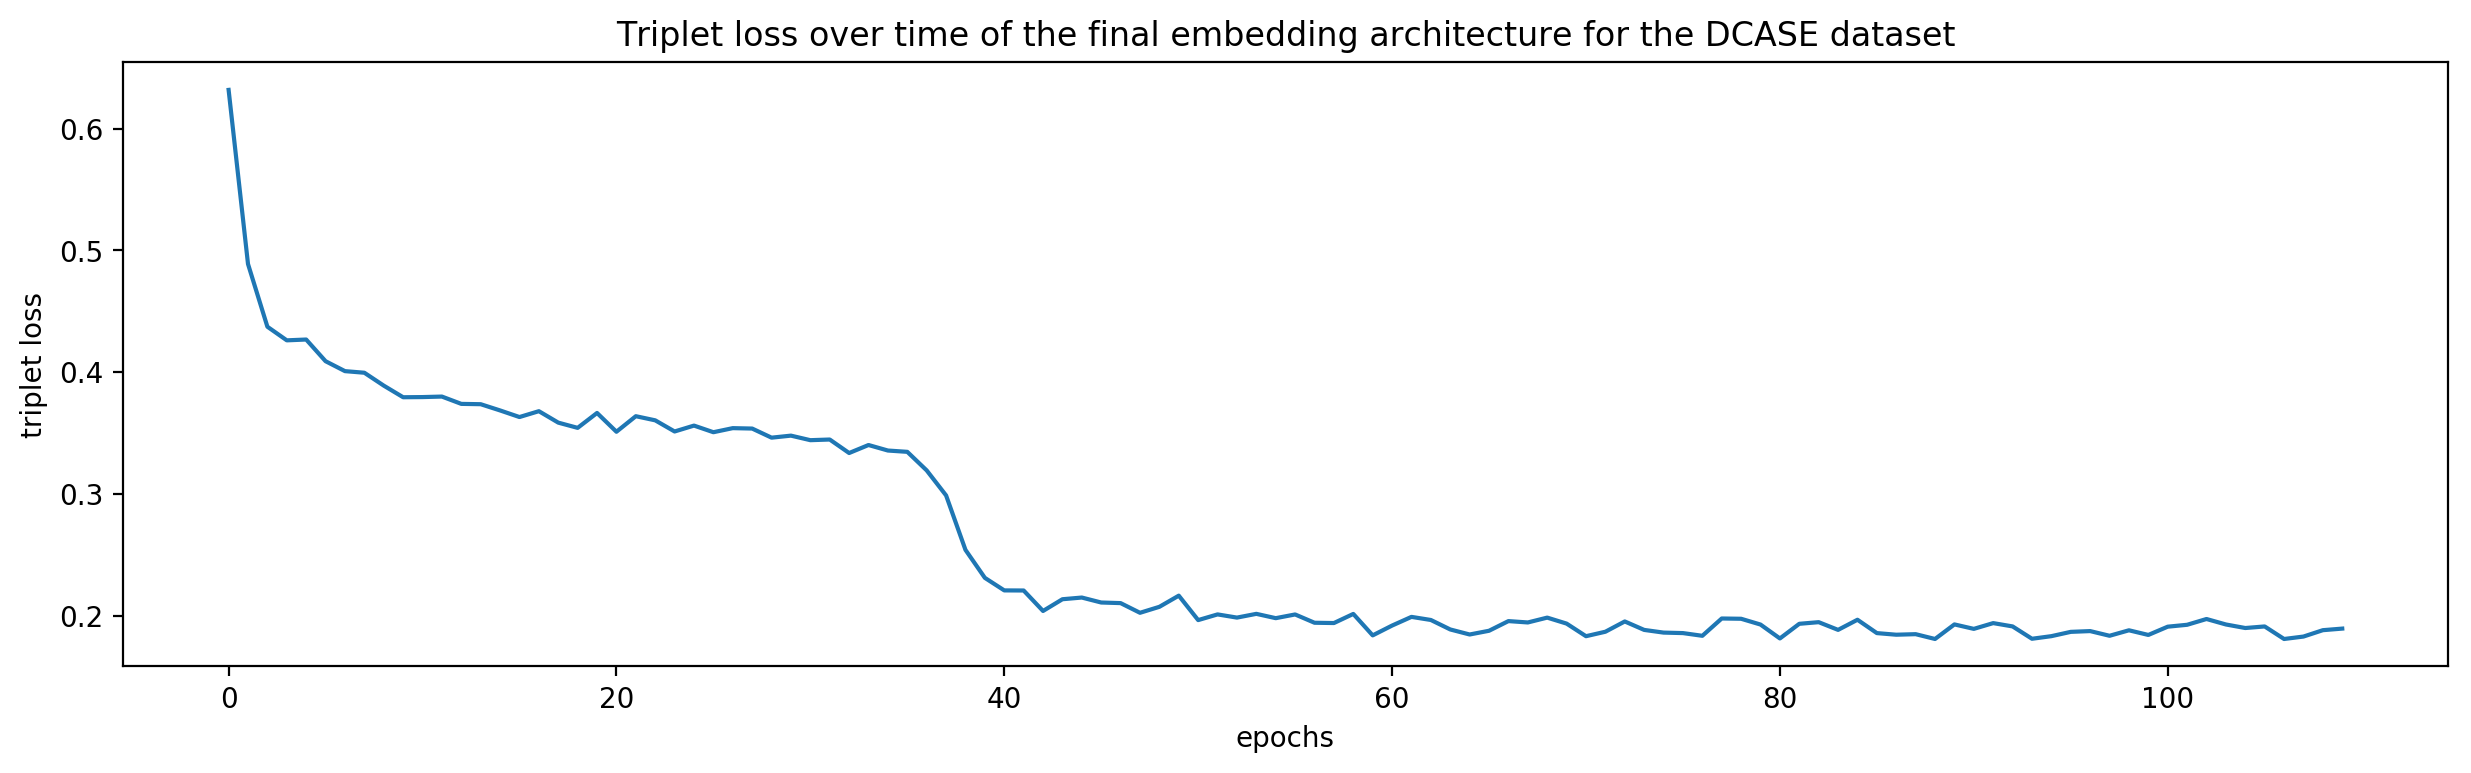
\includegraphics[width=0.6\linewidth]{img/Triplet_loss_DCASE_final.png}
    \caption{Triplet loss plot of the final embedding model for the noise detection dataset}
    \label{fig:Triplet-Loss-DCASE}
\end{figure}
\noindent
The optimal embedding space architecture for the \gls{DCASE} task 5 challenge in this thesis is given by the hyperparameters in table \ref{tab:Hyperparameters-DCASE} as well as in table \ref{tab:Hyperparameters-Detailed-DCASE}, which shows the hyperparameters in more detail. Most of the parameters in the list result out of the conducted experiments. However, the ones who did not result out of an experiment are default ones proposed by the organizers of the \gls{DCASE} challenge. The margin resulted out of the margin experiment \ref{sub:Experiment-Margin}, the regularisation factor out of the regularisation experiment \ref{sub:Experiment-Regularisation-Factor}, the embedding dimension from the experiment \ref{sub:Experiment-Embedding-Size} and \ref{sub:Experiment-Larger-Embedding-Sizes}, the sample segment size from the experiment \ref{sub:Experiment-Segment-Size} and the feature extractor from the experiment \ref{sub:Experiment-Feature-Representation}. The batch size was chosen to be the highest possible value without getting an out of memory exception. With more extensive computing resources, a larger batch size could be used, and the model would almost surely only benefit from it.
\newline
\newline
The model was trained for 110 epochs until convergence and reached a triplet loss value of 0.1879, which is by far the lowest loss of all the different experiments. The triplet loss value is shown in figure \ref{fig:Triplet-Loss-DCASE}. The plot shows that the model has decreased a significant amount between the 34 and the 39 epoch and afterwards started to converge.

\subsection{Embedding space}
\label{sub:Eval-Embedding-Space-DCASE}
The embedding space was further examined to get detailed insights about the resulting clusters and the distances between them.  The entire development dataset was projected onto the embedding space and saved, including with the corresponding label, name and segment, to examine the embedding space. Afterwards the embedding space was converted into an \texttt{cKDTree} from \texttt{scipy}, which is a kd-tree for quick nearest-neighbor lookup. This tree was used to get the neighbours from a specific data point in the embedding space. It uses the Euclidean distance (\ref{eq:Euclidean-Distance}) to calculate the distances between the points in the embedding space. The Euclidean distance is used because, in the triplet loss function (\ref{eq:Triplet-Loss}), this measurement is used to compare the distances between the triplets and therefore, it makes sense to use the same when calculating the neighbours.
\newline
\newline
First, the miss-classified embeddings were further examined, this is done by looping over the entire embedding space and checking if the label of the selected embedding and 20 of its neighbours are all different. If that is so, the segment and its neighbours are further examined. The examination showed that most of the segments which belong to a different cluster as their label, consisted of a big part of silence or were purely silence, and were therefore projected to the region of silence. Most of these segments consisted of a part of silence, and after for example, seven seconds a sound was observed. However, when segmenting each audio in segments, there is a high possibility, that the segment only consists of silence. This shows that the embedding space clusters the segments by their meaning and not by their activity, which means that silence when performing, for example, the activity \textit{working} or \textit{eating}, will be projected in the near-by region. It was also observed that there are a lot of audios, which do not contain any sound and are therefore purely silence but have the label \textit{working}. These audio files should be examined further because there is a chance that they are miss-classified and should be assigned to the label \textit{absence}. However, it can be reasoned, that silence when performing the activity \textit{working} belongs to the activity, since there is a high possibility that the person does not make any sound but the model should still recognise this activity as \textit{working}. Nevertheless, this provided useful insights into the dataset as well as the embedding space. It was also observed that there are some audios, where a microphone malfunction is present and because of that are wrong classified, for example audio \texttt{DevNode3\_ex53\_42}.
\newline
\newline
The other examination of the embedding space focused on the correct classified segments and aimed to show the nature of the embedding space. The idea is to select two labels of the dataset, for example, \textit{working} and \textit{eating}, then to loop over the dataset and checking if the embedding belongs to one of these classes and further has five neighbours from the same label. If this is the case, the embedding will be appended to a list of the corresponding label. These lists are then used to calculate the mean of the clusters from each label. The checking of the neighbourhood of each embedding is used to neglect the problem of outliers in clusters. Afterwards, the distance between the clusters is calculated and divided by a specified number of steps, which indicates how many steps have to be taken to reach the other label. Then the centroid of the first label is taken, and the step difference is added to it. From this position, the nearest neighbours are taken and displayed. This process is repeated until the position of the other centroid label is reached. This \flqq walk through the embedding space\frqq can then be represented as an image (\ref{fig:Walk-through-DCASE}) or as a continuous recording of the segments appended with each other. This representation shows that the embedding space represents much meaning because when walking through the space, for example from \textit{working} to \textit{social\_activity} the figure \ref{fig:Walk-through-DCASE} shows that there is more sound activity when approaching \textit{social\_activity}. However this increase is done in a rather slow matter and for example in the figure \ref{fig:Walk-through-DCASE}, the line three represents audios from \textit{social\_activity} where there is still a lot of silence or quiet talking.
\begin{figure}[ht]
\centering
    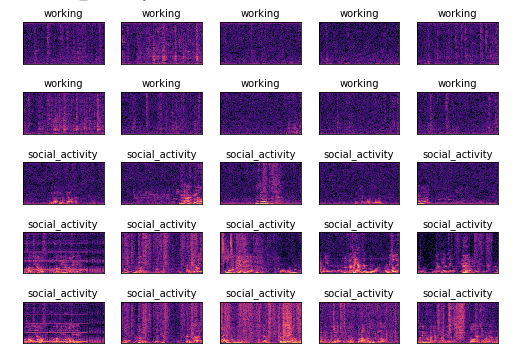
\includegraphics[width=0.8\linewidth]{img/Walk_through_dcase_space.png}
    \caption{\flqq walk through the embedding space\frqq \ of the DCASE space from \textit{working} to \textit{social\_activity}}
    \label{fig:Walk-through-DCASE}
\end{figure}

\subsection{Comparison to challenge results}
\label{sub:Eval-Comparison-DCASE}
One of the primary evaluations for the embedding space is how well a simple logistic classifier, which is trained on top of the embedding space, performs. The metrics of the classifier are used to compare and evaluate different embedding spaces and also to compare how well it performs in comparison to the models submitted in the \gls{DCASE} task 5 challenge. The submitted architectures were compared using the F1 score of the evaluation dataset using. The main goal of the challenge was to show that models are able to recognise daily activities using different microphone arrays. Therefore, to compare the models in the challenge, the F1 score was calculated from the evaluation set where the microphones were unknown and were not present in the training dataset. The winner of the challenge was a team from IBM, which accomplished an F1 score on the unknown microphones of 88.4\% and a 90.4\% F1 score on the entire evaluation dataset. The embedding space in this thesis was only compared using the full evaluation dataset.
\newline
\newline
On the final embedding architecture for this challenge, described in \ref{sub:Eval-Embedding-Space-DCASE}, the trained classifier accomplished a macro-averaged F1 score of 62.19\% on the full evaluation dataset. The difference between the results of this thesis and the challenge is approximately 30\% to the winner and 20\% to the others. A detailed classification report is given by figure \ref{fig:classification-report-DCASE}, which shows the precision, recall and F1-score of each class. It can be seen that the classes \textit{other} and \textit{eating} are the hardest to classify. This is mainly due to the nature of their sounds and the high imbalance in the dataset. The class \textit{other} is used when an activity is performed, which does not belong to a label in the dataset and therefore contains a lot of different sounds. The label \textit{eating} is very hard to differentiate, because the sound of eating itself is very similar to \textit{dish washing} or \textit{cooking} since there are mainly noises of kitchen utilities present.
\begin{figure}[ht]
\centering
    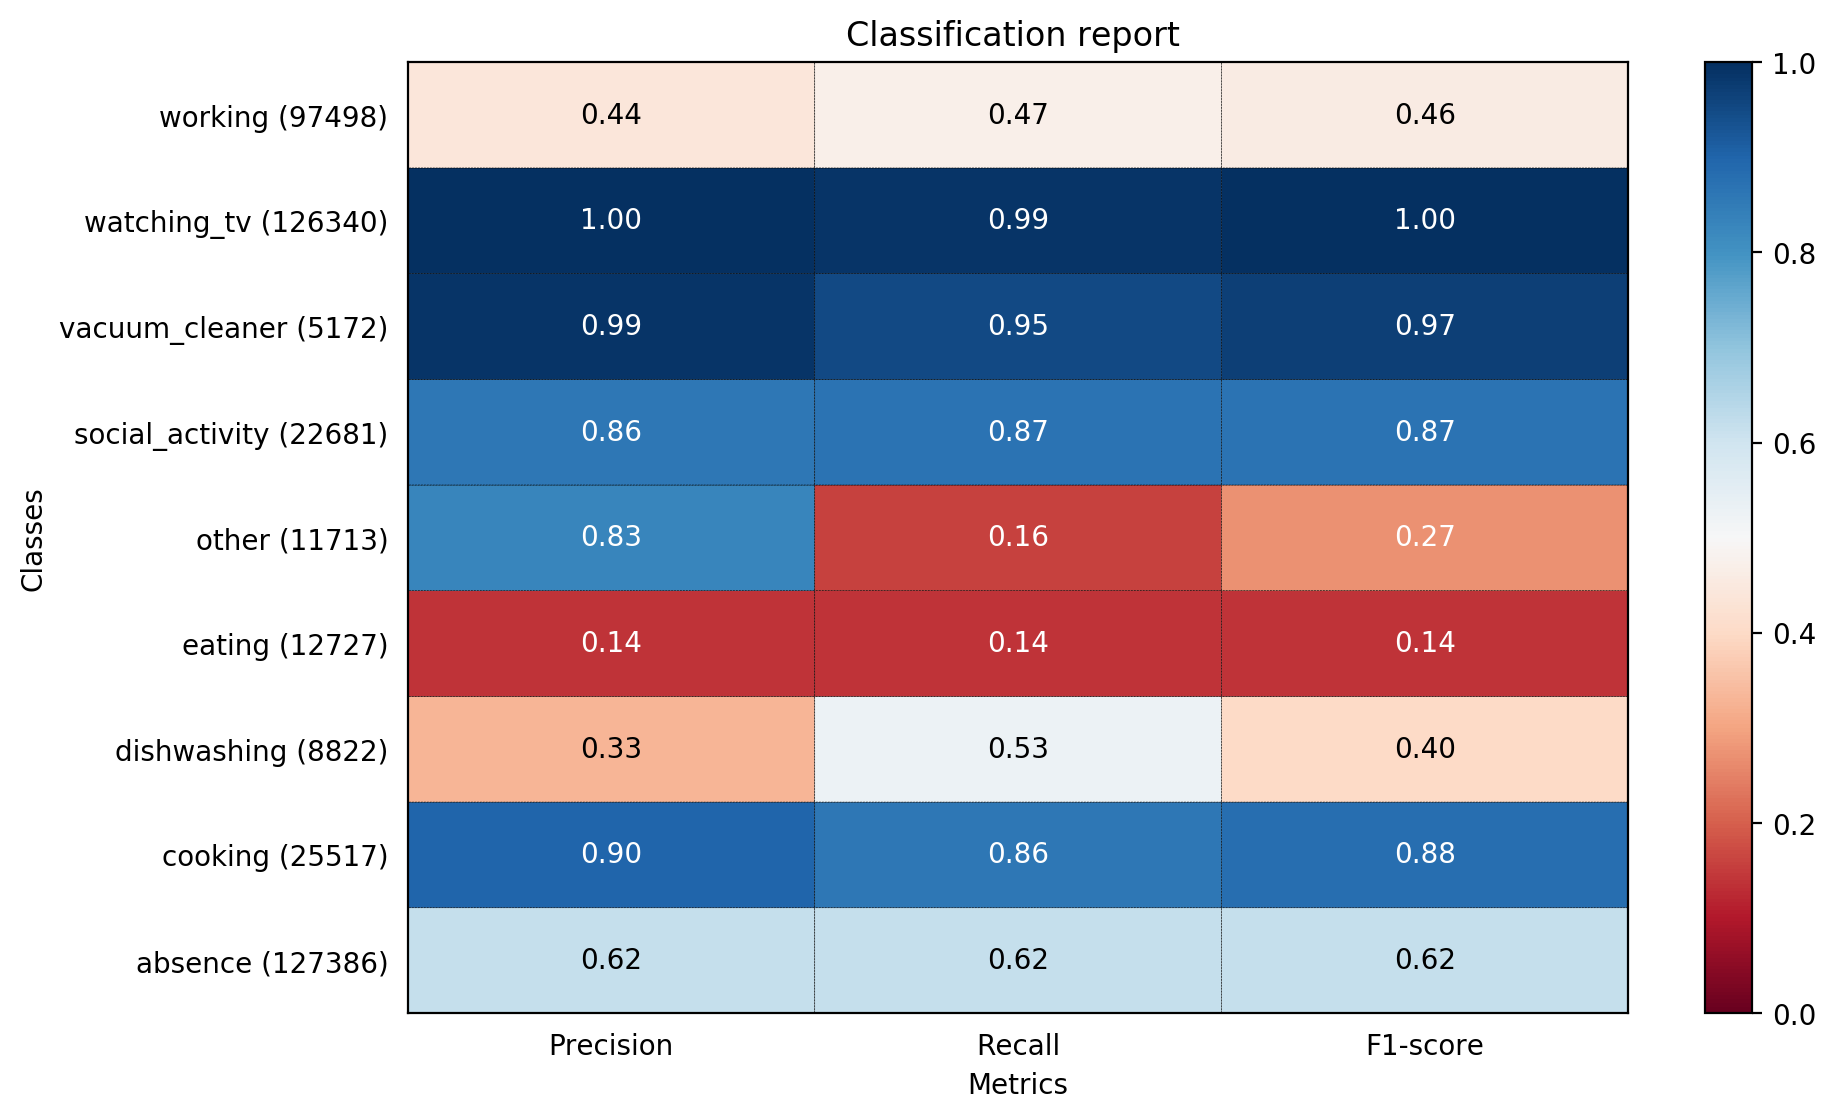
\includegraphics[width=0.8\linewidth]{img/DCASE_F1_classification_report.png}
    \caption{Classification report of the classifier on the evaluation dataset from the DCASE challenge}
    \label{fig:classification-report-DCASE}
\end{figure}

\subsection{Conclusion}
\label{sub:Eval-Conclusion-DCASE}
The results from the examination of the embedding space for the \gls{DCASE} challenge are quite astonishing since the embedding space represents much meaning, such as the distribution of the clusters and miss-classified segments are off place. It is fascinating that all of this meaning can be extracted purely based on the nature of the sound rather than the underlying label. One of the most astonishing properties of the embedding space is that it can find miss-classified audios or even microphone malfunctions within the dataset. 
\newline
\newline
However, when comparing the model to the challenge results, the embedding space performs not so well, which means that there is a 20\% gap between the trained embedding model and the challenge results. Nevertheless, since the goal was not to beat the participants in the challenge, but rather to create an embedding space which represents meaning and the comparison to the challenge was only used to show the difference between the approaches, the accomplished results compared to the challenge are still good. Furthermore, if a more extensive architecture, such as a ResNet, would be trained on top of the embedding space, the results could be profoundly improved.
\newline
\newline
The resulting embedding model uses a state-of-the-art ResNet18 architecture, which resulted in good results. More massive architectures such as ResNet50 or ResNet152 were not evaluated due to the lack of time and resources. Other approaches, such as \gls{CRNN}, should also be evaluated to find the optimal state-of-the-art architecture. There is a possibility that using more massive architectures would result in a better embedding space since there are more weights available. However, the possibility of overfitting also increases. Nevertheless, experiments have to show how the embedding space varies when increasing the architecture and if there is a performance gain when doing so.

\section{Music dataset}
\label{sec:Results-Music}
This section describes the results of the experiments with the music dataset (\ref{sub:Music-Dataset}). The intention was to show that the created embedding space is applicable not only to the noise detection domain but can be used throughout the audio domain. The intention of using the embedding space was the same as for the \gls{DCASE} challenge dataset, to create an embedding space where distances represent the similarity between segments. When using the music dataset, this similarity between sound segments can then be used to find similar segments or to cluster segments by similarity. This section shows the examination of the embedding space to test if the model succeeded finding similarities, by first examining the embedding space manually (\ref{sub:Results-Music-Embedding-Space}), then by applying a clustering (\ref{sub:Results-Music-Clustering}) and then finally by conducting a qualitative analysis in the form of an interview with mister Emanuel Oehri (\ref{sub:Results-Music-Qualitative-analysis}). The final part of this section is to provide a conclusion about the models' performance on the music dataset (\ref{sub:Results-Music-Conclusion}).

\subsection{Resulting model}
\label{sub:Results-Music-Resulting-Model}
\begin{table}[ht]
    \centering
    \caption{Hyperparameters of the optimal embedding architecture for the music dataset}
	\label{tab:Hyperparameters-Music}
    \begin{tabular}{l|l}
        \toprule
        \textbf{Hyperparameter} & \textbf{value} \\ 
        \midrule[1pt]
        Model & ResNet18 \\ 
        \hline
        Epochs & 130 \\ 
        \hline
        Batch size & 32 \\ 
        \hline
        Optimizer & Adam \\ 
        \hline
        Learning rate & 1e-5 \\
        \hline
        Margin & 1.0 \\
        \hline
        L2 regularisation factor & 0.01 \\
        \hline
        Embedding dimension & 256 \\
        \midrule[1pt]
        \multicolumn{2}{l}{\textit{Audio sample}} \\
        \midrule[1pt]
        Sample rate & 44100 \\ 
        \hline
        Sample segment size & 10s \\
        \hline
        Sample segment range & 40s \\
        \hline
        Convert to mono & True \\
        \midrule[1pt]
        \multicolumn{2}{l}{\textit{Feature representation}} \\
        \midrule[1pt]
        Feature extractor & LogMelExtractor \\ 
        \hline
        Input size & 998 x 128 \\
        \bottomrule
    \end{tabular}
\end{table}
\noindent
The same embedding architecture as the one for the noise detection dataset, with mostly the same hyperparameters, was used. The hyperparameters for the music dataset are given by table \ref{tab:Hyperparameters-Music} and table \ref{tab:Hyperparameters-Detailed-Music}, which shows the hyperparameters in more detail. The difference in the hyperparameters is mainly due to the different structure of the dataset and their audio samples. In the \gls{DCASE} challenge dataset, the samples are already split into 10s segments, whereas the samples in the music dataset are full songs of a specific genre, which leads to variable audio lengths in the dataset. However, this does not make any difference in the input pipeline but instead gives an additional possibility to split the samples into larger segments. The experiment with the different segment sizes (\ref{sub:Experiment-Segment-Size}), showed that using larger segments results in much clearer clusters and therefore, in a better embedding space. Therefore the segment size was increased from 5s to 10s, which further resulted in a two times larger input size. This further led to the decrease of the batch size to 32, because of the initial batch size led to an out of memory exception due to the lack of larger computational resources. The increase of the neighbouring range is as well because there is the possibility of doing so due to the nature of the samples of the dataset. The increase provides a vaster possibility of triplet combinations, which the model can only profit from.
\newline
\newline
The resulting model was trained for 130 epochs, which took around seven and a half days, the training took this long, mainly because the triplet selection ant therefore also the splitting of the song was done on the fly in the input pipeline. The training process could be significantly decreased when using \texttt{TFRecords}\footnote{\href{https://www.tensorflow.org/tutorials/load\_data/tfrecord\#tfrecord\_files\_using\_tfdata}{www.tensorflow.org/tutorials/load\_data/tfrecord}}. However the conversion of the dataset to \texttt{TFRecords} was neglected since this would provide a more static dataset, rather than a more dynamic one. If the dataset is more dynamic, the model learns to handle differences in the dataset a lot better, since the dataset is continually changing and therefore focuses more on the underlying structure of each segment. However, this leads to models which need to be trained a lot longer than with a more static dataset.
\newline
\newline
The figure \ref{fig:Triplet-Loss-Music} shows the graph of the triplet loss value of the trained epochs. It shows that the model starts with a relatively high loss value and decreases over time. At the end of the training, at epoch 130, the model reached a triplet loss value of approximately 0.35. The graph further shows that the model could potentially profit from additional training with a lower learning rate to get an even lower triplet loss value.
\begin{figure}[ht]
\centering
    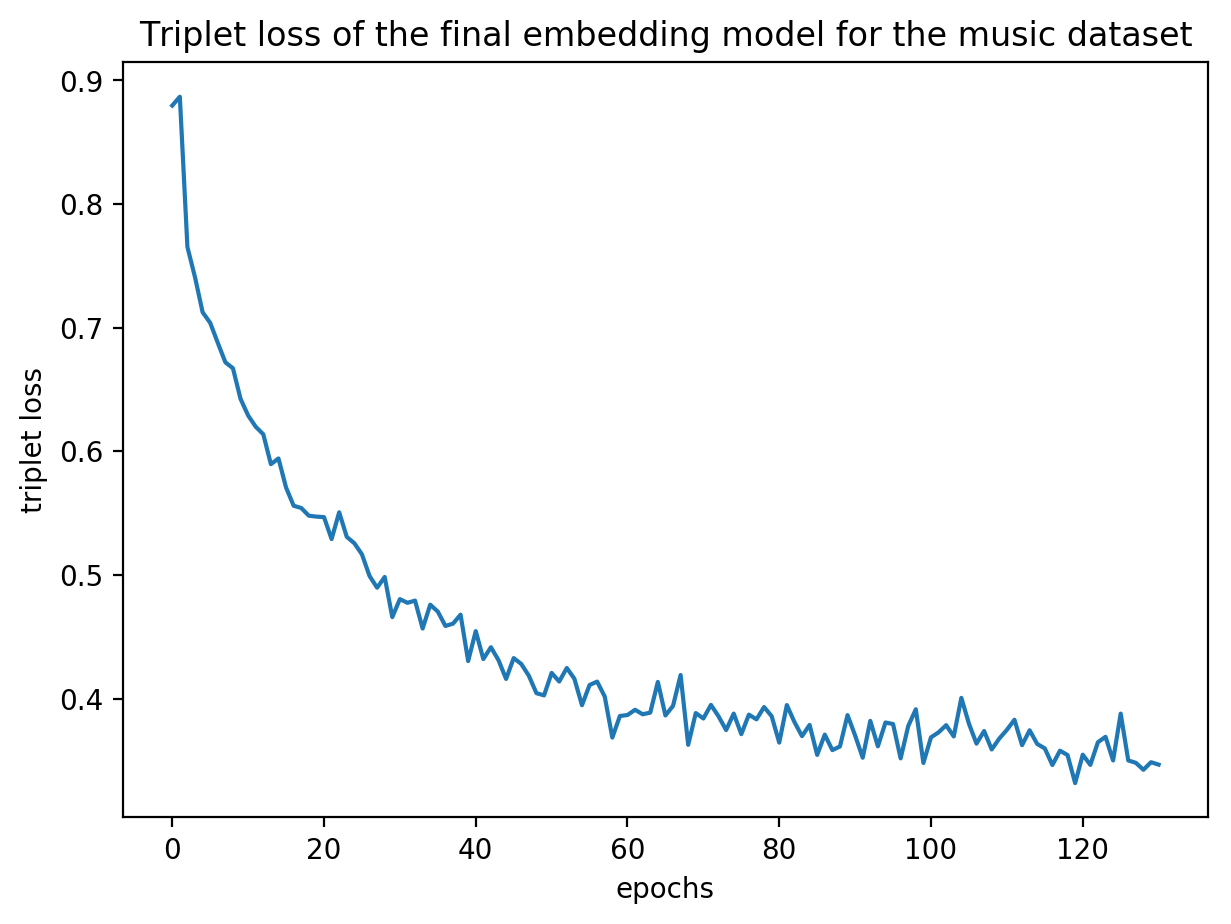
\includegraphics[width=0.6\linewidth]{img/triplet_loss_music_final.png}
    \caption{Triplet loss plot of the final embedding model for the music dataset}
    \label{fig:Triplet-Loss-Music}
\end{figure}

\subsection{Embedding space}
\label{sub:Results-Music-Embedding-Space}
\begin{figure}[ht]
\centering
    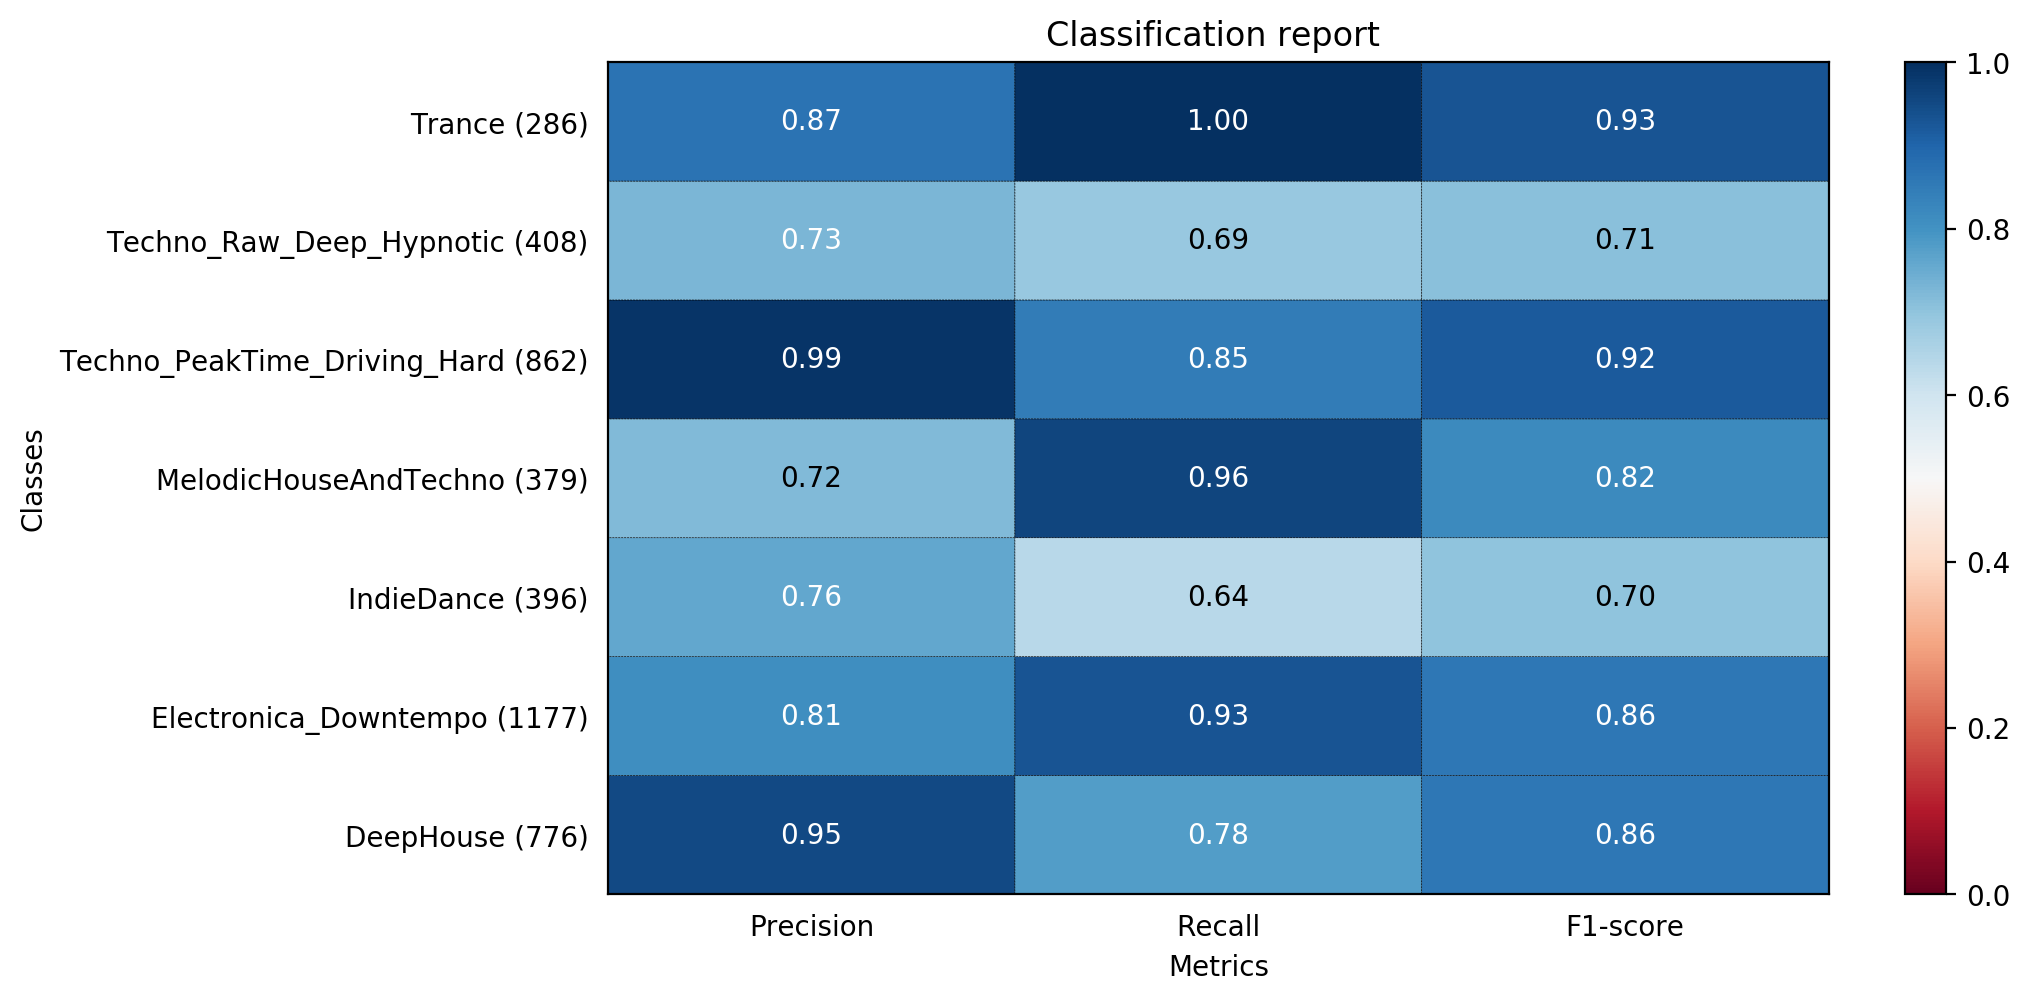
\includegraphics[width=0.9\linewidth]{img/music_plot_classif_report.png}
    \caption{Classification report of the classifier trained on the music dataset}
    \label{fig:Classification-Report-Muisc}
\end{figure}
\noindent
The music embedding space was similarly examined as the noise detection space (\ref{sub:Eval-Embedding-Space-DCASE}). For the examination, the entire dataset was projected onto the embedding space and the value, including the metadata of each point, was saved. The examination was done in a jupyter notebook located in the \texttt{notebooks} folder called \texttt{examination\_embedding\_space.ipynb}.
\newline
\newline
Similar as for the evaluation of the noise detection embedding space, the same logistic classifier was trained using embedded audio segments as input, which aimed to show how easy a classifier can separate the clusters in the embedding space by only fitting hyperplanes in it. The classifier was trained using the same hyperparameters as the resulting model (\ref{sub:Results-Music-Resulting-Model}) for 40 epochs and accomplished a macro-averaged F1 score of 84\%. The detailed classification report is shown in figure \ref{fig:Classification-Report-Muisc}.
\newline
\newline
The first part of the examination was to explore the neighbourhood of the embedding space, which was done by building a neighbouring tree using the \texttt{cKDTree} from \texttt{scipy}. The \texttt{cKDTree} uses the Euclidean distance (\ref{eq:Euclidean-Distance}) to calculate the distances between the points in the embedding space. The Euclidean distance is used because, in the triplet loss function (\ref{eq:Triplet-Loss}), this measurement is used to compare the distances between the triplets and therefore, it makes sense to use the same when calculating the neighbours. Then to examine the neighbourhood, from each of the embedded points its nearest 30 neighbours were checked, and their labels were compared, which aims to find inconsistencies. If a sample had 28 or more different labels in its neighbourhood, it was further examined, since this represents either a malfunction of the embedding space or a significant sample in the dataset, which can be classified as a different genre. These points were then appended with its five nearest neighbours and a song was created, which represents the neighbourhood. This song showed that even if the neighbourhood was inconsistent, the resulting sound did still sound very similar to an amateur. However, since this needs to be evaluated by an expert, these generated songs were used in the qualitative analysis (\ref{sub:Results-Music-Qualitative-analysis}) and evaluated by a professional DJ.
\newline
\newline
The next examination of the embedding space was to compute the centroids of each category cluster, and then taking the five nearest neighbours from each, which will then be used to create a song from all of the segments. This created song should represent a typical song of the specific cluster. For an amateur this it sounds like this is the case, however, this needs to be shown in the qualitative analysis (\ref{sub:Results-Music-Qualitative-analysis}).
\newline
\newline
The last examination of the embedding space was walking through the embedding space, which was already done and described in the section above from the noise detection dataset (\ref{sub:Eval-Embedding-Space-DCASE}). The idea is to walk from cluster to cluster with a specified amount of steps and taking the three next neighbours from each one of the steps. All of the audios were then appended and a this results in a song, which should represent a song with the starting point in a specific cluster and then ends in a different one, where the transitions should sound reasonable. This \flqq walk through the embedding space\frqq \ can further be represented as an image, where the log Mel representation is computed of each of the segments and then appended as a sub-figure to the overall figure. Such an image is shown in figure \ref{fig:Walk-through-Music}. The figure shows, that when purely looking at it, the transitions seem reasonable and a clear build up was noticed to the label \textit{Trance}. However, this needs to be shown in the qualitative analysis (\ref{sub:Results-Music-Qualitative-analysis}) as well. Each combination of categories was computed and the resulting song with the corresponding image of the \flqq walk through the embedding space\frqq \ was saved.
\begin{figure}[ht]
\centering
    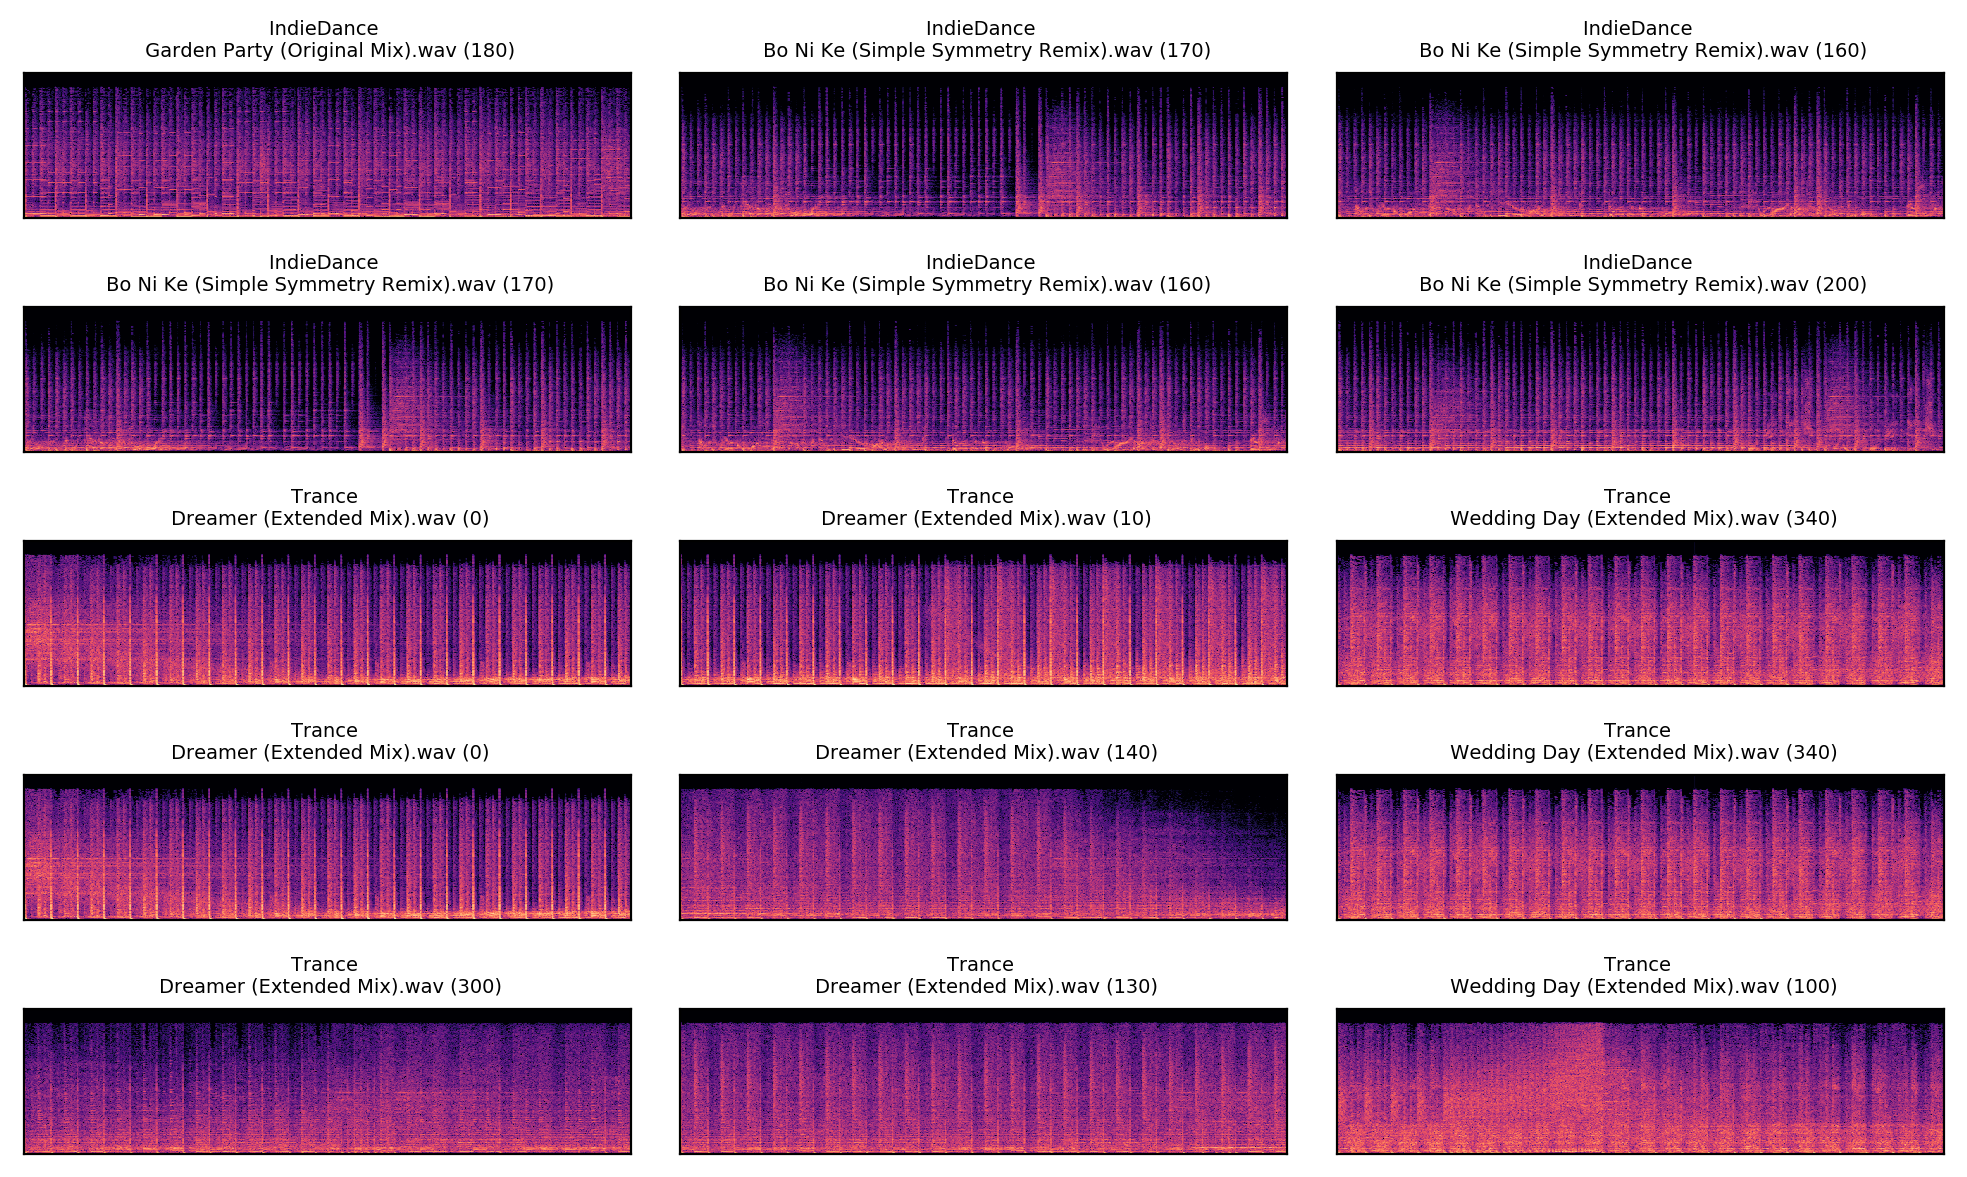
\includegraphics[width=0.9\linewidth]{img/Walk_through_music_space.png}
    \caption{\flqq walk through the embedding space\frqq \ of the music space from \textit{IndieDance} to \textit{Trance}}
    \label{fig:Walk-through-Music}
\end{figure}

\subsection{Clustering applied to embedding space}
\label{sub:Results-Music-Clustering}
\begin{figure}[ht]
\centering
    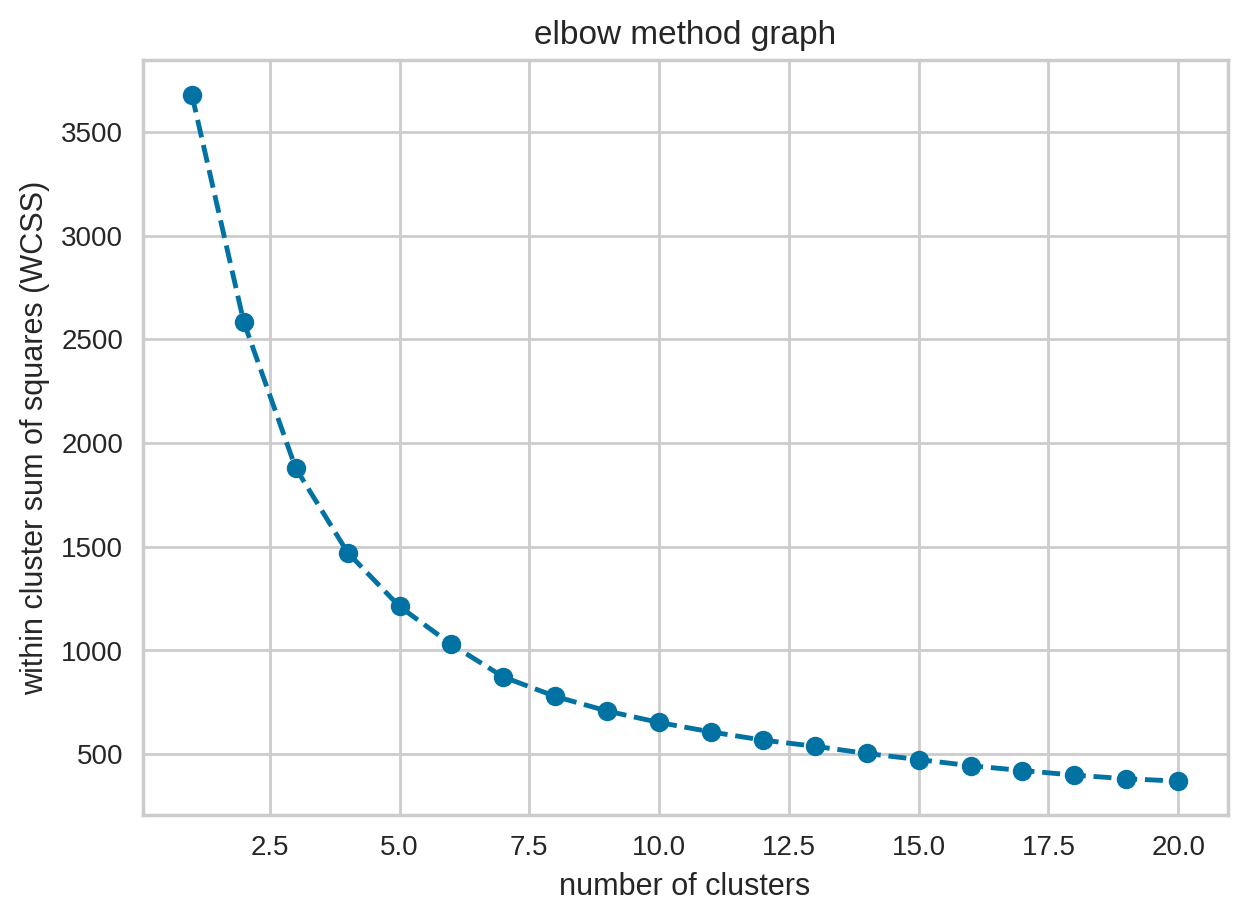
\includegraphics[width=0.6\linewidth]{img/elbow_method_music_dataset.png}
    \caption{Plot of the elbow method on the music embedding space to find the optimal number of clusters}
    \label{fig:Elbow-Clusters}
\end{figure}
\noindent
One of the requirements of the thesis was to apply a standard clustering algorithm to the embedding space and examining the resulting clusters. For this thesis, K-Means is chosen as the clustering algorithm (\ref{sub:K-Means}), since clustering was explicitly excluded from the thesis and only a simple and easy to implement algorithm should be used. To apply clustering to the embedding space and to visualise the results, the dimensionality had to be reduced to at least three dimensions. The dimensionality reduction was done by computing \gls{PCA} and using only three principal components. Afterwards, these three principal components were used to compute the \gls{WCSS} with equation \ref{eq:Objective-Function-K-Means}, for the different number of clusters, with results in computing the elbow method, which is used to find the optimal number of clusters. The \gls{WCSS} measures the average squared distance of all the points within a cluster to the cluster centroid. Figure \ref{fig:Elbow-Clusters} shows the plot of the \gls{WCSS} when increasing the number of clusters. The figure shows that the optimal number of classes is between six and seven because this represents the \flqq elbow\frqq \ of the graph. For this evaluation, the optimal number of clusters is chosen to be seven, since this was also the number of different sub-genres in the dataset. Thereafter, K-Means was computed using seven clusters by using the implementation of \texttt{sklearn}. When visualising the cluster, this results in the figure \ref{fig:K-Means-Visualisation}, where the colours represent the clusters and the \flqq x\frqq \ represents the centre of each cluster.
\newline
\newline
The resulting clusters were examined by looking at the distribution of the different labels contained in each. This aims to show which cluster contains which labels. Table \ref{tab:Distribution-KMeans-Clusters} shows the distribution of each of the seven clusters. The clustering result shows that in every cluster, there is a different sub-genre which occurs most frequently. This shows that even with such a simple clustering algorithm, there are separated clusters of each of the seven sub-genres. However, the clusters still contain a fair amount of different labels, which is typical in such entangled categories as the ones in the music dataset.
\begin{figure}[ht]
\centering
    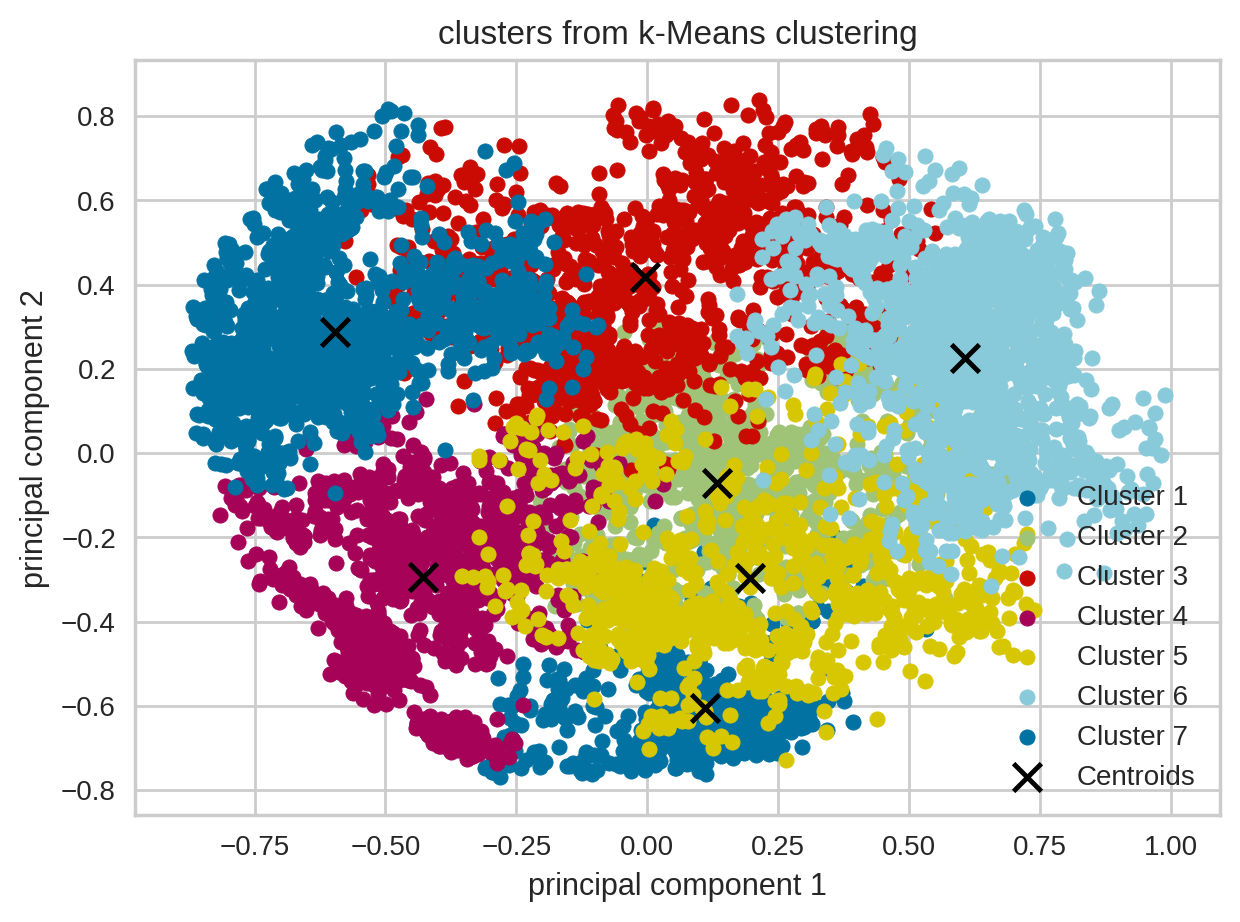
\includegraphics[width=0.8\linewidth]{img/kmeans_music.png}
    \caption{K-Means visualisation of the embedding space}
    \label{fig:K-Means-Visualisation}
\end{figure}
\begin{table}[htbp]
    \centering
    \caption{Distribution of the sub-genres in each one of the seven clusters computed with K-Means}
	\label{tab:Distribution-KMeans-Clusters}
    \begin{tabular}{l|l}
        \toprule
        \textbf{cluster id} & \textbf{sub-categories (count of each)} \\ 
        \midrule[1pt]
        1 & \begin{minipage}{4in}
        \vskip 4pt
        MelodicHouseAndTechno (28) \\
        Techno\_Raw\_Deep\_Hypnotic (54) \\
        Trance (711)
        \vskip 4pt
        \end{minipage} \\ 
        \hline
        2 & \begin{minipage}{4in}
        \vskip 4pt
        DeepHouse (183) \\
        Electronica\_Downtempo (139) \\
        IndieDance (451) \\
        MelodicHouseAndTechno (362) \\
        Trance (31)
        \vskip 4pt
        \end{minipage} \\
        \hline
        3 & \begin{minipage}{4in}
        \vskip 4pt
        DeepHouse (395) \\
        Electronica\_Downtempo (112) \\
        IndieDance (99) \\
        MelodicHouseAndTechno (209) \\
        Techno\_PeakTime\_Driving\_Hard (105) \\
        Techno\_Raw\_Deep\_Hypnotic (86) \\
        Trance (115)
        \vskip 4pt
        \end{minipage} \\
        \hline
        4 & \begin{minipage}{4in}
        \vskip 4pt
        DeepHouse (93) \\
        Electronica\_Downtempo (164) \\
        IndieDance (165) \\
        Techno\_PeakTime\_Driving\_Hard (49) \\
        Techno\_Raw\_Deep\_Hypnotic (521) \\
        Trance (62)
        \vskip 4pt
        \end{minipage} \\
        \hline
        5 & \begin{minipage}{4in}
        \vskip 4pt
        DeepHouse (101) \\
        Electronica\_Downtempo (625) \\
        IndieDance (43) \\
        MelodicHouseAndTechno (91) \\
        Techno\_Raw\_Deep\_Hypnotic (53) 
        \vskip 4pt
        \end{minipage} \\
        \hline
        6 & \begin{minipage}{4in}
        \vskip 4pt
        DeepHouse (373) \\
        Electronica\_Downtempo (36) \\
        IndieDance (300) \\
        MelodicHouseAndTechno (644) 
        \vskip 4pt
        \end{minipage} \\
        \hline
        7 & \begin{minipage}{4in}
        \vskip 4pt
        IndieDance (34) \\
        MelodicHouseAndTechno (55) \\
        Techno\_PeakTime\_Driving\_Hard (975) \\
        Techno\_Raw\_Deep\_Hypnotic (174) \\
        Trance (91)
        \vskip 4pt
        \end{minipage} \\
        \bottomrule
    \end{tabular}
\end{table}

\subsection{Qualitative analysis}
\label{sub:Results-Music-Qualitative-analysis}
The qualitative analysis aims to evaluate the embedding space created for music, with the help of an expert. In this thesis, the expert is mister Emanuel Oehri, which is a DJ and also kindly provided the music dataset and therefore is very familiar with the sub-genres of the dataset, since he picked these out. In the following subsection, Emanuel Oehri will be referred to as the expert. The qualitative analysis was done in the form of an interview, where the interview guide can be found in the appendix \ref{sec:Interview-Guide}. The key elements of the analysis were summarised and described in this subsection. The detailed interview can be found in the appendix \ref{sec:Interview-Answers}.
\newline
\newline
First, the songs of each cluster centre were evaluated with the expert. The process of calculating these combined songs are described in \ref{sub:Results-Music-Embedding-Space}. The expert pointed out that the songs represent the underlying category very well. However, he further mentioned, that the song of the category \textit{DeepHouse} after 30 seconds sounded much more typical than the other segments, which indicates that there is still some noise even in the cluster centres of each sub-category.
\newline
\newline
Second, the expert evaluated the songs which did not have a consistent neighbourhood from the section \ref{sub:Results-Music-Embedding-Space} and he mentioned, that even though the category of them are different, they sound very similar and their similarity is reasonable. He then further pointed out that some of the songs, which had an inconsistent neighbourhood, were from the start or the end of a song. This indicates that the embedding space succeeds in embedding the middle part of the songs correctly, which is evident since this part of the song represents its genre much better than a start or an end. However, he also found some segments in the songs, which would probably fit better in another cluster.
\newline
\newline
Together with the expert, some of the distances and calculations between the clusters were examined, and a few interesting ones were found. Such as the ones shown in \ref{eq:Subtracting-Adding-Clusters-Music}. These few equations show that the embedding space succeeded to find some similarity or dissimilarity between the genres. It further indicates, that the position of each cluster in the embedding space has a meaning behind it, which can further be used to compute the similarities between them. However, from 42 of these combinations computed, only four of them represented correct properties. 
\myequations{Subtracting and adding distances of cluster centers in the music embedding space}
\begin{equation}
    \centering
    \begin{split}
        &\text{IndieDance} - \text{Techno\_Raw\_Deep\_Hypnotic} = \text{DeepHouse} \\
        &\text{DeepHouse} - \text{Electronica\_Downtempo} = \text{MelodicHouseAndTechno} \\
        &\text{DeepHouse} - \text{IndieDance} = \text{Electronica\_Downtempo}
    \end{split}
    \label{eq:Subtracting-Adding-Clusters-Music}
\end{equation}
Further, the clusters resulting from k-Means were examined by the expert mainly with the focus of the combination of each clusters' sub-genres. For the expert, the combinations of sub-genres within each cluster made much sense, even though these were sometimes a bit noisy. The most important criteria when evaluating these clusters was that each cluster must have a significantly higher amount of a specific class within it. This criterion was satisfied for all of the seven clusters in the embedding space.
\newline
\newline
When examining the \flqq walk through the embedding space\frqq \ the expert pointed out that some of the transitions, mostly from very different sub-genres, were not very smooth or contained some segments, which did not fit as well as the others. However, when looking at the \flqq walk\frqq \ between somewhat similar categories, the transitions sounded very interesting (in a good way) for the expert.
\newline
\newline
Overall the expert was very impressed with the achieved results since the identified similarities made complete sense for him. He mentioned that it was more like finding the flaws rather than finding good properties. He then further mentioned, that he would consider the experiment to be a success, since that the embedding space succeeded in finding similarities between songs even if they are not in the same category but still, in fact, sounds very similar. The expert found some of the transitions between the sub-genre very impressive and could imagine playing these in a live DJ set.

\subsection{Conclusion}
\label{sub:Results-Music-Conclusion}
The examination of the embedding space for the music dataset showed some significant properties, such as that it succeeded in finding similarities in even such entangled sub-genres, which are quite impressive. Further, the examination showed that the embedding space successfully built seven clusters for each of the sub-genres. Each one of these clusters still contains segments of other categories. However, this is evident, since the goal of the project was to find the underlying structure of the data, rather than to classify the genres correctly. In the interview with mister Emanuel Oehri, he mentioned, that the genre can be chosen by the label itself when uploading the song, which means that there is also the possibility that a song which is labelled as one category, would, in fact, better belong into a different category.
\newline
\newline
Nevertheless, during the examination, a few flaws of the embedding space were found. One of which is that the embedding space has problems when it comes to embedding the start or the end of a song, which further states that the embedding space has great difficulty in finding useful similarities in these segments of the song. This is mainly because at the start or the end of a song, the main characteristics of the genre are not present or only very limited. This problem could be solved, when using larger segments than 10 seconds, which provides even more information and therefore would result in an even better embedding space. Another way to solve this issue would be to train the model even longer with a lower learning rate and check if the model after this extensive learning period succeeds in learning to cluster the starting and ending segments of a song.
\newline
\newline
Another weakness of the embedding space is that the transitions between genres, which are relatively different from each other, such as \textit{Electronica\_Downtempo} and \textit{Trance}, are not as smooth as some others. This problem can be solved, if a more extensive dataset would be used, maybe with even more genres, which would provide the embedding space with more songs to smoothen the transitions. Another possibility would be to check if the transitions would benefit when using larger segments to train the model.
\newline
\newline
Further, it is to note, that the resulting clusters, when applying k-Means (\ref{fig:K-Means-Visualisation}) to the embedding space, still contains a lot of noise. This noise can result, because either the embedding space looks like that or because such a simple clustering algorithm is used to find the clusters in the embedding space. If for example, \gls{TSNE} would be used to visualise the clusters, it would result in much a clearer separation. Therefore, in future research, a more extensive clustering technique should be evaluated and used to visualise the resulting embedding space and resulting clusters. 
